% presentation
\documentclass{beamer}
\usetheme[height=7mm]{Rochester}
\usecolortheme{rose}

% handout

%\documentclass[handout]{beamer}
%\usepackage{pgfpages} \pgfpagesuselayout{8 on 1}[a4paper]

%\documentclass[mathserif]{article}
%\usepackage{beamerarticle}

\usepackage{amsmath}
\usepackage{comment}
\usepackage{amssymb,amsfonts}
\usepackage[T1]{fontenc}
\usepackage{lmodern}
\usepackage{tikz}
%\usepackage{simpsons}
\usepackage{marvosym}
\usepackage{color}
\usepackage{multirow}
\usepackage{pgffor}
\usepackage{pgfplots}
\usepackage[slide,algoruled,titlenumbered,vlined,noend,linesnumbered,]{algorithm2e}

\usefonttheme{structurebold}

\setbeamertemplate{footline}[frame number]
\setbeamertemplate{navigation symbols}{}
\setbeamerfont{smallverb}{size*={73}}
\usefonttheme[onlymath]{serif}
\setbeamertemplate{theorems}[numbered]
\newtheorem{construction}[theorem]{Construction}
\newtheorem{proposition}[theorem]{Proposition}

\AtBeginSection[] {
  \begin{frame}
    \frametitle{Content}
    \tableofcontents[currentsection]
  \end{frame}
  \addtocounter{framenumber}{-1}
}

\usetikzlibrary[shapes.arrows]
\usetikzlibrary{shapes.geometric}
\usetikzlibrary{backgrounds}
\usetikzlibrary{positioning}
\usetikzlibrary{calc}
\usetikzlibrary{intersections}
\usetikzlibrary{fadings}
\usetikzlibrary{decorations.footprints}
\usetikzlibrary{patterns}
\usetikzlibrary{shapes.callouts}
\usetikzlibrary{fit}
%handout

\providecommand{\abs}[1]{\lvert#1\rvert}

\tikzset{every picture/.style={line width=1pt,show background rectangle},background rectangle/.style={fill=blue!10,rounded corners=2ex}}

\newcommand{\Bob}[3]{ \begin{scope}[shift={(#1,#2)},scale=#3]
  \draw (0,0) circle (0.95 and 1);
  \fill (-0.3,-0.1) circle (0.1);
  \fill (+0.3,-0.1) circle (0.1);
  \draw (0.35,-0.5) arc (-70:-110: 1 and 0.4);
  \draw (-0.3,0.5) arc (-10:-80: 0.8 and 0.8);
  \draw (-0.5,0.8) arc (190:255: 2 and 1);
  \draw (-0.7,0.9) -- +(0.2,-0.09) -- +(0.25,0.2);
  \end{scope} }

\newcommand{\Alice}[3]{ \begin{scope}[shift={(#1,#2)},scale=#3]
  \draw (0,0) circle (0.95 and 1);
  \fill (-0.3,-0.1) circle (0.1);
  \fill (+0.3,-0.1) circle (0.1);
  \draw (0.35,-0.5) arc (-70:-110: 1 and 0.4);
  \draw (0.3,1.3) arc (20:-100: 1.4 and 1);
  \draw (0.5,1.3) arc (150:260: 1 and 1);
  \draw (0.41,1.3) circle (0.35);
  \end{scope} }

  \newcommand{\Evil}[3]{ \begin{scope}[shift={(#1,#2)},scale=#3]
    \draw (0,0) circle (0.95 and 1);
    \fill (-0.1,-0.1) -- +(-0.2,-0.1) -- +(-0.4,0.2); %eye
    \fill (0.1,-0.1) -- +(0.2,-0.1) -- +(0.4,0.2);
    \draw (0.35,-0.5) arc (-70:-110: 1 and 0.4);
    %\fill (0.3,-0.5) -- +(-0.1,-0.2) -- +(-0.2,-0.02);
    %\fill (-0.3,-0.5) -- +(0.1,-0.2) -- +(0.2,-0.02);
    \fill (0.3,0.7) -- +(0.5,0.4) -- +(0.4,-0.2); % horn
    \fill (-0.3,0.7) -- +(-0.5,0.4) -- +(-0.4,-0.2);
    %\draw (0.3,1.3) arc (20:-100: 1.4 and 1);
    %\draw (0.5,1.3) arc (150:260: 1 and 1);
    %\draw (0.41,1.3) circle (0.35);
    \end{scope} }

\newcommand{\Charlie}[3]{ \begin{scope}[shift={(#1,#2)},scale=#3]
    \draw (0,0) circle (0.95 and 1);
    \filldraw[fill=black!20] (-0.35,-0.1) circle (0.25);
    \filldraw[fill=black!20] (+0.35,-0.1) circle (0.25);
    %\draw (0.9,0.2) to [bend left] (-0.9,0.2);
    \draw (0.2,0) to [bend left] (-0.2,0);


    %\draw (0.3,0.7) to [bend right] (-0.3,0.7);
    %\draw (0.4,0.5) to [bend right] (-0.4,0.5);
    %\draw (0.35,-0.5) arc (-70:-110: 1 and 0.4);
    \draw (-0.7,-0.6) to [bend right] (0,-0.6) to [bend right] (0.7,-0.6) to [bend right]  (0,-0.5)  to [bend right]  cycle ;
    %\draw (0.3,1.3) arc (20:-100: 1.4 and 1);
    %\draw (0.5,1.3) arc (150:260: 1 and 1);
    %\draw (0.41,1.3) circle (0.35);
    \end{scope} }

\author{Yu Zhang}
\institute{Harbin Institute of Technology}
\date[Crypto'22A]{Cryptography, Autumn, 2022}

%% presentation
\documentclass{beamer}
\usetheme[height=7mm]{Rochester}
\usecolortheme{rose}

% handout

%\documentclass[handout]{beamer}
%\usepackage{pgfpages} \pgfpagesuselayout{8 on 1}[a4paper]

%\documentclass[mathserif]{article}
%\usepackage{beamerarticle}

\usepackage{amsmath}
\usepackage{comment}
\usepackage{amssymb,amsfonts}
\usepackage[T1]{fontenc}
\usepackage{lmodern}
\usepackage{tikz}
%\usepackage{simpsons}
\usepackage{marvosym}
\usepackage{color}
\usepackage{multirow}
\usepackage{pgffor}
\usepackage{pgfplots}
\usepackage[slide,algoruled,titlenumbered,vlined,noend,linesnumbered,]{algorithm2e}

\usefonttheme{structurebold}

\setbeamertemplate{footline}[frame number]
\setbeamertemplate{navigation symbols}{}
\setbeamerfont{smallverb}{size*={73}}
\usefonttheme[onlymath]{serif}
\setbeamertemplate{theorems}[numbered]
\newtheorem{construction}[theorem]{Construction}
\newtheorem{proposition}[theorem]{Proposition}

\AtBeginSection[] {
  \begin{frame}
    \frametitle{Content}
    \tableofcontents[currentsection]
  \end{frame}
  \addtocounter{framenumber}{-1}
}

\usetikzlibrary[shapes.arrows]
\usetikzlibrary{shapes.geometric}
\usetikzlibrary{backgrounds}
\usetikzlibrary{positioning}
\usetikzlibrary{calc}
\usetikzlibrary{intersections}
\usetikzlibrary{fadings}
\usetikzlibrary{decorations.footprints}
\usetikzlibrary{patterns}
\usetikzlibrary{shapes.callouts}
\usetikzlibrary{fit}
%handout

\providecommand{\abs}[1]{\lvert#1\rvert}

\tikzset{every picture/.style={line width=1pt,show background rectangle},background rectangle/.style={fill=blue!10,rounded corners=2ex}}

\newcommand{\Bob}[3]{ \begin{scope}[shift={(#1,#2)},scale=#3]
  \draw (0,0) circle (0.95 and 1);
  \fill (-0.3,-0.1) circle (0.1);
  \fill (+0.3,-0.1) circle (0.1);
  \draw (0.35,-0.5) arc (-70:-110: 1 and 0.4);
  \draw (-0.3,0.5) arc (-10:-80: 0.8 and 0.8);
  \draw (-0.5,0.8) arc (190:255: 2 and 1);
  \draw (-0.7,0.9) -- +(0.2,-0.09) -- +(0.25,0.2);
  \end{scope} }

\newcommand{\Alice}[3]{ \begin{scope}[shift={(#1,#2)},scale=#3]
  \draw (0,0) circle (0.95 and 1);
  \fill (-0.3,-0.1) circle (0.1);
  \fill (+0.3,-0.1) circle (0.1);
  \draw (0.35,-0.5) arc (-70:-110: 1 and 0.4);
  \draw (0.3,1.3) arc (20:-100: 1.4 and 1);
  \draw (0.5,1.3) arc (150:260: 1 and 1);
  \draw (0.41,1.3) circle (0.35);
  \end{scope} }

  \newcommand{\Evil}[3]{ \begin{scope}[shift={(#1,#2)},scale=#3]
    \draw (0,0) circle (0.95 and 1);
    \fill (-0.1,-0.1) -- +(-0.2,-0.1) -- +(-0.4,0.2); %eye
    \fill (0.1,-0.1) -- +(0.2,-0.1) -- +(0.4,0.2);
    \draw (0.35,-0.5) arc (-70:-110: 1 and 0.4);
    %\fill (0.3,-0.5) -- +(-0.1,-0.2) -- +(-0.2,-0.02);
    %\fill (-0.3,-0.5) -- +(0.1,-0.2) -- +(0.2,-0.02);
    \fill (0.3,0.7) -- +(0.5,0.4) -- +(0.4,-0.2); % horn
    \fill (-0.3,0.7) -- +(-0.5,0.4) -- +(-0.4,-0.2);
    %\draw (0.3,1.3) arc (20:-100: 1.4 and 1);
    %\draw (0.5,1.3) arc (150:260: 1 and 1);
    %\draw (0.41,1.3) circle (0.35);
    \end{scope} }

\newcommand{\Charlie}[3]{ \begin{scope}[shift={(#1,#2)},scale=#3]
    \draw (0,0) circle (0.95 and 1);
    \filldraw[fill=black!20] (-0.35,-0.1) circle (0.25);
    \filldraw[fill=black!20] (+0.35,-0.1) circle (0.25);
    %\draw (0.9,0.2) to [bend left] (-0.9,0.2);
    \draw (0.2,0) to [bend left] (-0.2,0);


    %\draw (0.3,0.7) to [bend right] (-0.3,0.7);
    %\draw (0.4,0.5) to [bend right] (-0.4,0.5);
    %\draw (0.35,-0.5) arc (-70:-110: 1 and 0.4);
    \draw (-0.7,-0.6) to [bend right] (0,-0.6) to [bend right] (0.7,-0.6) to [bend right]  (0,-0.5)  to [bend right]  cycle ;
    %\draw (0.3,1.3) arc (20:-100: 1.4 and 1);
    %\draw (0.5,1.3) arc (150:260: 1 and 1);
    %\draw (0.41,1.3) circle (0.35);
    \end{scope} }

\author{Yu Zhang}
\institute{Harbin Institute of Technology}
\date[Crypto'22A]{Cryptography, Autumn, 2022}

%\input{1introduction.tex}
%\input{2perfectlysecret.tex}
%\input{3privatekey.tex}


\title{Introduction}

\begin{document}
\maketitle
\begin{frame}
\frametitle{Outline}
\tableofcontents
\end{frame}
\section{Cryptography and Modern Cryptography}
\begin{frame}\frametitle{What is Cryptography?}
\begin{itemize}
\item \textbf{Cryptography}: from Greek \emph{krypt\'os}, ``hidden, secret''; and \emph{gr\'{a}phin}, ``writing''
\item \textbf{Cryptography}: the art of writing or solving codes.\\ (Concise oxford dictionary 2006)
\item \textbf{Codes}: a system of prearranged signals, especially used to ensure secrecy in transmitting messages. \\ (\emph{code word} in cryptography)
\item \textbf{1980s}: from Classic to Modern; from Military to Everyone
\item \textbf{Modern cryptography}: the scientific study of mathematical techniques for securing digital information, systems, and distributed computations against adversarial attacks
\end{itemize}
\end{frame}
\begin{frame}\frametitle{What is cryptography? [xkcd:504]}
\begin{figure}
\begin{center}
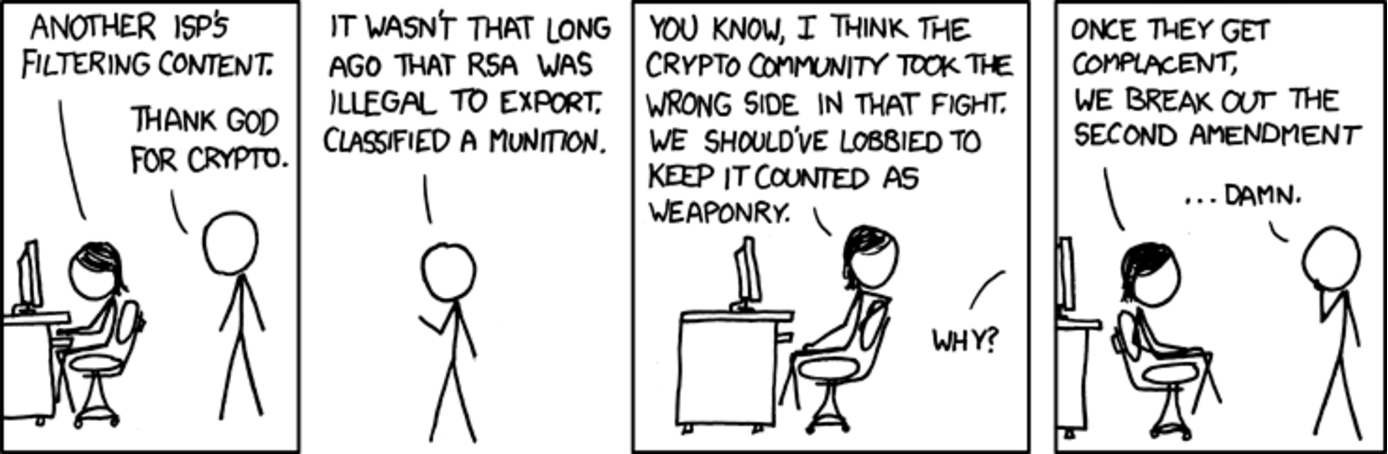
\includegraphics[width=100mm]{pic/legal} 
\end{center}
\end{figure}
\end{frame}
\section{The Setting of Private-Key Encryption}
\begin{frame}\frametitle{Private-Key Encryption}
\begin{itemize}
\item \textbf{Goal}: to construct \textbf{ciphers} (encryption schemes) for providing secret communication between two parties sharing \textbf{private-key} (the symmetric-key) in advance
\item \textbf{Implicit assumption}: there is some way of initially sharing a key in a secret manner
\item \textbf{Disk encryption}: the same user at different points in time
\end{itemize}
\end{frame}
\begin{frame}\frametitle{Alice, Bob  [xkcd:1323]}
Changing the names would be easier, but if you're not comfortable lying, try only making friends with people named Alice, Bob, Carol, etc.
\begin{figure}
\begin{center}
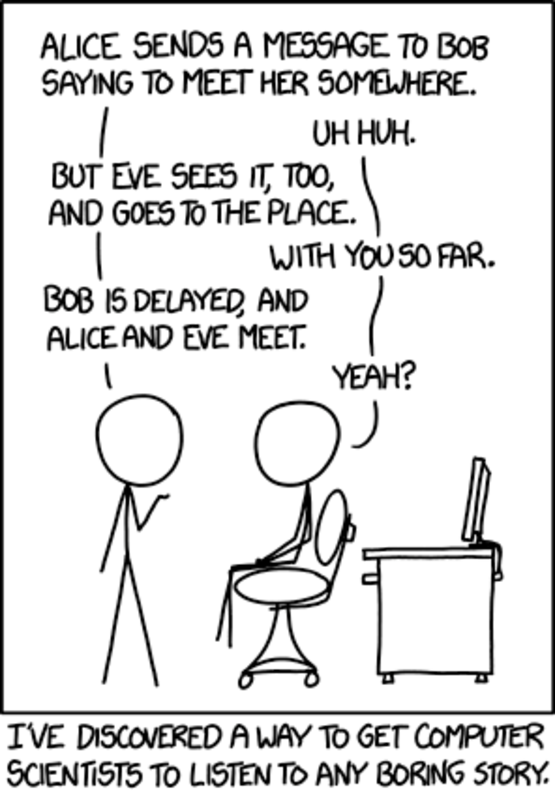
\includegraphics[width=45mm]{pic/alice-bob} 
\end{center}
\end{figure}
\end{frame}
\begin{frame}\frametitle{The Syntax of Encryption}
\begin{figure}
\begin{center}
\begin{tikzpicture}
\node (sender) [minimum size=1cm] {}; \Alice{0}{0}{0.4};
\node (bart) [below of = sender, node distance = 0.7cm] {Alice};
\node (enc) [draw, right of = sender, rounded corners=1ex,node distance = 2cm] {$\mathsf{Enc}$};
\node (k1) [above of = enc, node distance = 1cm] {$k$};
\node (c) [right of = enc, node distance = 2cm] {$c$};
\node (gen) [draw, above of = c, rounded corners=1ex,node distance = 1cm] {$\mathsf{Gen}$};
\node (adv) [below of = c, node distance = 1cm, minimum size=1cm] {}; \Evil{4cm}{-1cm}{0.4};
\node (burns) [below of = adv, node distance = 0.7cm] {Adversary};
\node (dec) [draw, right of = c, rounded corners=1ex,node distance = 2cm] {$\mathsf{Dec}$};
\node (k2) [above of = dec, node distance = 1cm] {$k$};
\node (receiver) [right of = dec, node distance = 2cm, minimum size=1cm] {}; \Bob{8cm}{0}{0.4};
\node (lisa) [below of = receiver, node distance = 0.7cm] {Bob};
\draw[-latex] (sender) -- (enc) node [midway, above] {$m$};
\draw (enc) -- (c); \draw[-latex] (c) -- (dec);
\draw[-latex] (dec) -- (receiver) node [midway, above] {$m$};
\draw[-latex] (k1) -- (enc);
\draw[-latex] (gen) -- (k1);
\draw[-latex] (gen) -- (k2);								
\draw[-latex] (k2) -- (dec);		
\end{tikzpicture}
\end{center}
\end{figure}
\begin{itemize}
\item key $k \in \mathcal{K}$, plaintext (or message) $m \in \mathcal{M}$, ciphertext $c \in \mathcal{C}$
\item \textbf{Key-generation} algorithm~$k \gets \mathsf{Gen}$
\item \textbf{Encryption} algorithm~$c:= \mathsf{Enc}_k(m)$
\item \textbf{Decryption} algorithm~$m:= \mathsf{Dec}_k(c)$
\item \textbf{Encryption scheme}: $\Pi = (\mathsf{Gen}, \mathsf{Enc}, \mathsf{Dec})$
\item \textbf{Basic correctness requirement}: $\mathsf{Dec}_k(\mathsf{Enc}_k(m)) = m$
\end{itemize}
\end{frame}
\begin{frame}\frametitle{Securing Key vs Obscuring Algorithm}
\begin{itemize}
\item Easier to maintain secrecy of a short key
\item In case the key is exposed, easier for the honest parties to change the key
\item In case many pairs of people, easier to use the same algorithm, but different keys
\end{itemize}
\begin{alertblock}{Kerckhoffs's principle}
\begin{quote}
The cipher method must not be required to be secret, and it must be able to fall into the hands of the enemy without inconvenience.
\end{quote}	
\end{alertblock}
\begin{alertblock}{Shannon's maxim}
	\begin{quote}
		The enemy knows the system.
	\end{quote}	
\end{alertblock}
\end{frame}
\begin{frame}\frametitle{Why ``Open Cryptographic Design''}
\begin{itemize}
\item Published designs undergo public scrutiny are to be stronger
\item Better for security flaws to be revealed by ``ethical hackers''
\item Reverse engineering of the code (or leakage by industrial espionage) poses a serious threat to security
\item Enable the establishment of standards.
\end{itemize}
\begin{exampleblock}{Dual EC: A Standardized Back Door}
	``Dual EC was standardized by NIST, ANSI, and ISO among other algorithms to generate pseudorandom numbers.'' ``The Snowden revelations, and in particular reports on Project Bullrun and the SIGINT Enabling Project, have indicated that Dual EC was part of a systematic effort by NSA to subvert standards.'' ``Reuters reported that NSA paid RSA ``\$10 million in a deal that set [Dual EC] as the preferred, or default, method for number generation in the BSafe software.''''	
\end{exampleblock}
\end{frame}
\begin{frame}\frametitle{Attack Scenarios}	
\begin{itemize}
\item \textbf{Ciphertext-only}: the adversary just observes ciphertext
\item \textbf{Known-plaintext}: the adversary learns pairs of plaintexts/ciphertexts under the same key
\item \textbf{Chosen-plaintext}: the adversary has the ability to obtain the encryption of plaintexts of its choice
\item \textbf{Chosen-ciphertext}: the adversary has the ability to obtain the decryption of \textbf{other} ciphertexts of its choice
\item \textbf{Passive attack}: COA KPA
\begin{itemize}
\item because not all ciphertext are confidential
\end{itemize}
\item \textbf{Active attack}: CPA CCA
\begin{itemize}
\item when to encrypt/decrypt whatever an adversary wishes?
\end{itemize}
\end{itemize}	
\end{frame}
\section{Historical Ciphers and Their Cryptanalysis}
\begin{comment}
	\begin{frame}\frametitle{Why We Learn Broken Ciphers?}
	\begin{itemize}
	\item To understand the weaknesses of an ``ad-hoc'' approach
	\item To learn that ``simple'' approaches are unlikely to succeed
	\item To feel that ``we are smart enough to do some crypt-analyzing''
	\end{itemize}
	\end{frame}
\end{comment}

\begin{frame}[fragile]\frametitle{Caesar's Cipher}
\begin{quote}
If he had anything confidential to say, he wrote it in cipher, that is, by so changing the order of the letters of the alphabet, that not a word could be made out. If anyone wishes to \alert{decipher} these, and get at their meaning, he must \alert{substitute the fourth letter of the alphabet, namely D, for A}, and so with the others

\rightline{--Suetonius,``Life of Julius Caesar''}
\end{quote}
\begin{itemize}
	\item $\mathsf{Enc}(m)=m+3\mod 26$ \footnote{In fact the quote indicates that decryption involved rotating letters of the alphabet forward 3 positions, $\mathsf{Dec}(c)=c+3\mod 26$}
	\item \textbf{Weakness}: ? %\alert{What is the key?}
\end{itemize}
\begin{exampleblock}{Example}
\verb|begintheattacknow|
%\verb|EHJLQWKHDWWDFNQRZ|
\end{exampleblock}
\end{frame}
\begin{frame}[fragile]\frametitle{Shift Cipher}
\begin{itemize}
\item $\mathsf{Enc}_k(m)=m+k\mod 26$
\item $\mathsf{Dec}_k(c)=c-k\mod 26$
\item \textbf{Weakness}: ? %Fragile under \textbf{Brute-force attack} (exhaustive search)
\end{itemize}
\begin{exampleblock}{Example: Decipher the string}	
\verb|EHJLQWKHDWWDFNQRZ|
\end{exampleblock}
\begin{alertblock}{Sufficient Key Space Principle}
Any secure encryption scheme must have a key space that is not vulnerable to exhaustive search.\footnote{If the plaintext space is larger than the key space.}
\end{alertblock}
\end{frame}
\begin{frame}\frametitle{Index of Coincidence (IC) Method (to find $k$)}
\textbf{How to automatically determine that the deciphered text makes sense?}

\textbf{Index of Coincidence (IC)}: the probability that two randomly selected letters (pick-then-return) will be identical.

Let $p_i$ denote the probability of $i$th letter in English text.
\[I \overset{\text{def}}{=}\sum_{i=0}^{25} p_i^2 \]
\begin{exampleblock}{Example}
What's the IC of `apple'?
\end{exampleblock}

For a long English text, the IC is $\approx 0.065$.
For $j = 0, 1, \dotsc , 25$, $q_j$ is the probability of $j$th letter in the ciphertext.
\[I_j \overset{\text{def}}{=}\sum_{i=0}^{25} p_i \cdot q_{i+j}\]
\alert{Q: For shift cipher, if $j = k$, then $I_j \approx$ ?}
\end{frame}

\begin{frame}[fragile]\frametitle{Mono-Alphabetic Substitution}
\begin{itemize}
\item \textbf{Idea}: To map each character to a different one in an arbitrary manner
\item \textbf{Strength}: Key space is large $\approx 2^{88}$. \alert{Q: how to count?}
\item \textbf{Weakness}: ? %The mapping of each letter is fixed
\end{itemize}
\begin{exampleblock}{Example}
\verb|abcdefghijklmnopqrstuvwxyz|\\
\verb|XEUADNBKVMROCQFSYHWGLZIJPT|

Plaintext: \verb|tellhimaboutme|\\
Ciphertext: \verb|??????????????|
\end{exampleblock}
\end{frame}
\begin{frame}[fragile]\frametitle{Attack with Statistical Patterns}
\begin{enumerate}
\item Tabulate the frequency of letters in the ciphertext
\item Compare it to those in English text
\item Guess the most frequent letter corresponds to \verb|e|, and so on
\item Choose the plaintext that does ``make sense'' (Not trivial)
\end{enumerate}
\begin{table}
\begin{center}
\caption{Average letter frequencies for English-language text}
\begin{tabular}{|cc|cc|cc|cc|cc|} \hline
e & 12.7\% & t & 9.1\% & a & 8.2\% & o & 7.5\% & i & 7.0\%\\
n & 6.7\% & \_ & 6.4\% & s & 6.3\% & h & 6.1\% & r & 6.0\%\\
d & 4.3\% & l & 4.0\% & c & 2.8\% & u & 2.8\% & m & 2.4\%\\
w & 2.4\% & f & 2.2\% & g & 2.0\% & y & 2.0\% & p & 1.9\%\\
b & 1.5\% & v & 1.0\% & k & 0.8\% & j & 0.2\% & x & 0.2\%\\
q & 0.1\% & z & 0.1\% & & & & & &\\ \hline
\end{tabular}
\end{center}
\end{table}
\end{frame}
\begin{frame}[fragile]\frametitle{Example of Frequency Analysis (Ciphertext)}
\begin{verbatim}
LIVITCSWPIYVEWHEVSRIQMXLEYVEOIEWHRXEXIPFEMVEWHKVS
TYLXZIXLIKIIXPIJVSZEYPERRGERIMWQLMGLMXQERIWGPSRIH
MXQEREKIETXMJTPRGEVEKEITREWHEXXLEXXMZITWAWSQWXSWE
XTVEPMRXRSJGSTVRIEYVIEXCVMUIMWERGMIWXMJMGCSMWXSJO
MIQXLIVIQIVIXQSVSTWHKPEGARCSXRWIEVSWIIBXVIZMXFSJX
LIKEGAEWHEPSWYSWIWIEVXLISXLIVXLIRGEPIRQIVIIBGIIHM
WYPFLEVHEWHYPSRRFQMXLEPPXLIECCIEVEWGISJKTVWMRLIHY
SPHXLIQIMYLXSJXLIMWRIGXQEROIVFVIZEVAEKPIEWHXEAMWY
EPPXLMWYRMWXSGSWRMHIVEXMSWMGSTPHLEVHPFKPEZINTCMXI
VJSVLMRSCMWMSWVIRCIGXMWYMX
\end{verbatim}
\end{frame}
\begin{frame}[fragile]\frametitle{Example of Frequency Analysis (Analysis)}
Count and Guess, Trial and Error.
\begin{table}
\begin{center}
\caption{Analysis Steps}
\begin{tabular}{|r|l|} \hline
Ciphertext & Plaintext \\ \hline
\alert{I}   & \alert{e} \\
\alert{XLI} & \alert{the} \\
\alert{E} & \alert{a} \\
\alert{R}tate & \alert{s}tate \\
atthatt\alert{MZ}e & atthatt\alert{im}e \\
he\alert{V}e & he\alert{r}e \\
remar\alert{A} & remar\alert{k} \\ \hline
\end{tabular}
\end{center}
\end{table}
\end{frame}
\begin{frame}[fragile]\frametitle{Example of Frequency Analysis (Plaintext)}
\begin{quote}
Hereupon Legrand arose, with a grave and stately air, and brought me the beetle
from a glass case in which it was enclosed. It was a beautiful scarabaeus, and, at
that time, unknown to naturalists -- of course a great prize in a scientific point
of view. There were two round black spots near one extremity of the back, and a
long one near the other. The scales were exceedingly hard and glossy, with all the
appearance of burnished gold. The weight of the insect was very remarkable, and,
taking all things into consideration, I could hardly blame Jupiter for his opinion
respecting it.

\rightline{--Edgar Allan Poe's ``The Gold-Bug''}
\end{quote}
\end{frame}

\begin{frame}[fragile]\frametitle{Vigen\`{e}re (poly-alphabetic shift) Cipher}
\begin{itemize}
\item \textbf{Idea}: To ``smooth out'' the distribution in the ciphertext by mapping different instances of the same letter in the plaintext to different ones in the ciphertext
\item \textbf{Encryption}: $c_i=m_i+k_{[i\bmod t]}$, $t$ is the length (period) of $k$
\item \textbf{Cryptanalysis}: Need find $t$; if $t$ is known, need know whether the decryption ``makes sense'', but brute force ($26^t$) is infeasible for $t > 15$
\end{itemize}
\begin{exampleblock}{Example (Key is `cafe')}
\begin{description}[Ciphertext]
\item[Plaintext]  \verb|tellhimaboutme| \\
\item[Key]        \verb|cafecafecafeca| \\
\item[Ciphertext] \verb|??????????????| %\verb|WFRQKJSFEPAYPF|
\end{description}
\end{exampleblock}
\end{frame}
\begin{frame}[fragile]\frametitle{Kasiski's Method (to find $t$)}
\begin{itemize}
\item To identify repeated patterns of length 2 or 3
\item The distance between such appearances is a multiple of $t$
\item $t$ is the greatest common divisor of all the distances
\end{itemize}
\begin{exampleblock}{Example (Key is `beads')}
\begin{semiverbatim}
themanandthewomanretrievedtheletterfromthepostoffice
beadsbeadsbeadsbeadsbeadsbeansdeadsbeadsbeadsbeadbea
VMFQTPFOH\alert{MJJ}XSFCSSIMTNFZXFYISEIYUIKHWPQ\alert{MJJ}QSLVTGJKGF
\end{semiverbatim}
\end{exampleblock}
\end{frame}
\begin{frame}\frametitle{Index of Coincidence (IC) Method (to find $t$)}
For $\tau = 1, 2, \dotsc$, $q_i$ is the probability of $i$th letter in $c_1, c_{1+\tau}, c_{1+2\tau}, \dotsc$, IC is
\[I_\tau \overset{\text{def}}{=}\sum_{i=0}^{25} q_i^2\]
\alert{If $\tau = t$, then $I_\tau \approx ?$} ; otherwise $q_i \approx \frac{1}{26}$ and
\[I_\tau \approx \sum_{i=0}^{25} \left(\frac{1}{26}\right)^2 \approx 0.038\]
Then reuse IC method to find $k_i$.
\begin{alertblock}{Arbitrary Adversary Principle}
Security must be guaranteed for any adversary within the class of adversaries having the specified power
\end{alertblock}
\end{frame}
\begin{frame}\frametitle{Cryptanalytic Attacks (homework assignment)}
\begin{itemize}
\item Under COA, the requirement for ciphertext related to the size of the key space.  Vig\`{e}nere > mono-alphabetic sub. > shift
\item Under KPA, trivially broken.
\end{itemize}
\begin{alertblock}{Lessons learned}
\begin{itemize}
\item Sufficient key space principle
\item Designing secure cipher is a hard task
\item Complexity does not imply security (then what does?)
\item Arbitrary adversary principle
\end{itemize}
\end{alertblock}
\end{frame}
\section{The Basic Principles of Modern Cryptography}
\begin{frame}\frametitle{Three Main Principles of Modern Cryptography}
\begin{enumerate}
\item The formulation of a rigorous \textbf{definition} of security / threat model
\item When the security of a cipher relies on an unproven \textbf{assumption}, this assumption must be precisely stated and be as minimal as possible
\item Cipher should be accompanied by a rigorous \textbf{proof} of security with the above definition and the above assumption
\end{enumerate}
\end{frame}
\begin{frame}\frametitle{Why Principle 1 -- Formulation of Exact Definitions}
\begin{exampleblock}{Q: how would you formalize the security for private-key encryption?}
\begin{enumerate}
\item \emph{No adversary can find the secret key when given a ciphertext.}\\
$\mathsf{Enc}_k(m)=m$
\item \emph{No adversary can find the plaintext that corresponds to the ciphertext.}\\
$\mathsf{Enc}_k(m)=m_{0}\| \mathsf{AES}_k(m)$
\item \emph{No adversary can determine any character of the plaintext that corresponds to the ciphertext.}\\
$m=1000$, someone can learn $ 800 < m < 1200$
\item \emph{No adversary can derive any meaningful information about the plaintext from the ciphertext.}\\
Could you define so-called `meaningful'?
\end{enumerate}
\emph{\alert{Definitions of security should suffice for all potential applications.}}
\end{exampleblock}
\end{frame}
\begin{frame}\frametitle{Why Principle 1 -- How to define}
%\begin{exampleblock}{General Form}
%A cryptographic scheme for a given \textbf{task} is secure if no adversary of a specified \textbf{power} can achieve a specified \textbf{break}
%\end{exampleblock}

How To Define Security -- Lesson From Alan Turing
\begin{itemize}
\item What's computation?\footnote{Q: Any ``mathematical proof that there exist well-defined problems that computers cannot solve''? A: Halting Problem in computability theory}
\begin{enumerate}
\item A direct appeal to \textbf{intuition}
\item A \textbf{proof of the equivalence} of two definitions\\ (The new one has a greater intuitive appeal)
\item Giving \textbf{examples} solved using a definition
\end{enumerate}
\item Additional method for security: \textbf{Test of time}
\end{itemize}
\end{frame}	
\begin{frame}\frametitle{Principle 2 -- Reliance on Precise Assumptions}
Most cryptographic constructions \textbf{cannot be proven secure unconditionally}
\begin{itemize}
	\item \textbf{Why?} 
	\begin{enumerate}
		\item Validation of the assumption
		\item Comparison of schemes
		\item Facilitation of proofs of security
	\end{enumerate}
	\textbf{The construction is secure if the assumption is true.}
	\item \textbf{How?} 
	\begin{enumerate}
		\item old, so well tested
		\item simple and lower-level, so easy to study, refute \& correct
	\end{enumerate}
\end{itemize}
\end{frame}
\begin{frame}\frametitle{Principle 3 -- Rigorous Proofs of Security}
\begin{itemize}
\item \textbf{Why?} Proofs are more desirable in computer security than in other fields.
\item \textbf{The reductionist approach}: 
\begin{theorem}	Given that Assumption X is true, Construction Y is secure according to the given definition.
\end{theorem}
\begin{proof} Reduce the problem given by X to the problem of breaking Y.
\end{proof}
\item \textbf{Ad-hoc approaches}: for those who need a ``quick and dirty'' solution, or who are just simply unaware.
\end{itemize}
\end{frame}
\begin{frame}\frametitle{Summary}
\begin{itemize}
\item Cryptography secures information, transactions and computations
\item Kerckhoffs's principle \& Open cryptographic design
\item Caesar's, shift, Mono-Alphabetic sub., Vigen\`{e}re
\item Brute force, letter frequency, Kasiski's, IC
\item Sufficient key space principle
\item Arbitrary adversary principle
\item Rigorously proven security
\end{itemize}
\end{frame}
\end{document}


%% presentation
\documentclass{beamer}
\usetheme[height=7mm]{Rochester}
\usecolortheme{rose}

% handout

%\documentclass[handout]{beamer}
%\usepackage{pgfpages} \pgfpagesuselayout{8 on 1}[a4paper]

%\documentclass[mathserif]{article}
%\usepackage{beamerarticle}

\usepackage{amsmath}
\usepackage{comment}
\usepackage{amssymb,amsfonts}
\usepackage[T1]{fontenc}
\usepackage{lmodern}
\usepackage{tikz}
%\usepackage{simpsons}
\usepackage{marvosym}
\usepackage{color}
\usepackage{multirow}
\usepackage{pgffor}
\usepackage{pgfplots}
\usepackage[slide,algoruled,titlenumbered,vlined,noend,linesnumbered,]{algorithm2e}

\usefonttheme{structurebold}

\setbeamertemplate{footline}[frame number]
\setbeamertemplate{navigation symbols}{}
\setbeamerfont{smallverb}{size*={73}}
\usefonttheme[onlymath]{serif}
\setbeamertemplate{theorems}[numbered]
\newtheorem{construction}[theorem]{Construction}
\newtheorem{proposition}[theorem]{Proposition}

\AtBeginSection[] {
  \begin{frame}
    \frametitle{Content}
    \tableofcontents[currentsection]
  \end{frame}
  \addtocounter{framenumber}{-1}
}

\usetikzlibrary[shapes.arrows]
\usetikzlibrary{shapes.geometric}
\usetikzlibrary{backgrounds}
\usetikzlibrary{positioning}
\usetikzlibrary{calc}
\usetikzlibrary{intersections}
\usetikzlibrary{fadings}
\usetikzlibrary{decorations.footprints}
\usetikzlibrary{patterns}
\usetikzlibrary{shapes.callouts}
\usetikzlibrary{fit}
%handout

\providecommand{\abs}[1]{\lvert#1\rvert}

\tikzset{every picture/.style={line width=1pt,show background rectangle},background rectangle/.style={fill=blue!10,rounded corners=2ex}}

\newcommand{\Bob}[3]{ \begin{scope}[shift={(#1,#2)},scale=#3]
  \draw (0,0) circle (0.95 and 1);
  \fill (-0.3,-0.1) circle (0.1);
  \fill (+0.3,-0.1) circle (0.1);
  \draw (0.35,-0.5) arc (-70:-110: 1 and 0.4);
  \draw (-0.3,0.5) arc (-10:-80: 0.8 and 0.8);
  \draw (-0.5,0.8) arc (190:255: 2 and 1);
  \draw (-0.7,0.9) -- +(0.2,-0.09) -- +(0.25,0.2);
  \end{scope} }

\newcommand{\Alice}[3]{ \begin{scope}[shift={(#1,#2)},scale=#3]
  \draw (0,0) circle (0.95 and 1);
  \fill (-0.3,-0.1) circle (0.1);
  \fill (+0.3,-0.1) circle (0.1);
  \draw (0.35,-0.5) arc (-70:-110: 1 and 0.4);
  \draw (0.3,1.3) arc (20:-100: 1.4 and 1);
  \draw (0.5,1.3) arc (150:260: 1 and 1);
  \draw (0.41,1.3) circle (0.35);
  \end{scope} }

  \newcommand{\Evil}[3]{ \begin{scope}[shift={(#1,#2)},scale=#3]
    \draw (0,0) circle (0.95 and 1);
    \fill (-0.1,-0.1) -- +(-0.2,-0.1) -- +(-0.4,0.2); %eye
    \fill (0.1,-0.1) -- +(0.2,-0.1) -- +(0.4,0.2);
    \draw (0.35,-0.5) arc (-70:-110: 1 and 0.4);
    %\fill (0.3,-0.5) -- +(-0.1,-0.2) -- +(-0.2,-0.02);
    %\fill (-0.3,-0.5) -- +(0.1,-0.2) -- +(0.2,-0.02);
    \fill (0.3,0.7) -- +(0.5,0.4) -- +(0.4,-0.2); % horn
    \fill (-0.3,0.7) -- +(-0.5,0.4) -- +(-0.4,-0.2);
    %\draw (0.3,1.3) arc (20:-100: 1.4 and 1);
    %\draw (0.5,1.3) arc (150:260: 1 and 1);
    %\draw (0.41,1.3) circle (0.35);
    \end{scope} }

\newcommand{\Charlie}[3]{ \begin{scope}[shift={(#1,#2)},scale=#3]
    \draw (0,0) circle (0.95 and 1);
    \filldraw[fill=black!20] (-0.35,-0.1) circle (0.25);
    \filldraw[fill=black!20] (+0.35,-0.1) circle (0.25);
    %\draw (0.9,0.2) to [bend left] (-0.9,0.2);
    \draw (0.2,0) to [bend left] (-0.2,0);


    %\draw (0.3,0.7) to [bend right] (-0.3,0.7);
    %\draw (0.4,0.5) to [bend right] (-0.4,0.5);
    %\draw (0.35,-0.5) arc (-70:-110: 1 and 0.4);
    \draw (-0.7,-0.6) to [bend right] (0,-0.6) to [bend right] (0.7,-0.6) to [bend right]  (0,-0.5)  to [bend right]  cycle ;
    %\draw (0.3,1.3) arc (20:-100: 1.4 and 1);
    %\draw (0.5,1.3) arc (150:260: 1 and 1);
    %\draw (0.41,1.3) circle (0.35);
    \end{scope} }

\author{Yu Zhang}
\institute{Harbin Institute of Technology}
\date[Crypto'22A]{Cryptography, Autumn, 2022}

%\input{1introduction.tex}
%\input{2perfectlysecret.tex}
%\input{3privatekey.tex}


\title{Perfectly Secret Encryption}

\begin{document}
\maketitle
\begin{frame}\frametitle{Outline}
\tableofcontents
\end{frame}
\section{Definitions and Basic Properties}
\begin{frame}\frametitle{Recall The Syntax of Encryption}
\begin{figure}
\begin{center}
\begin{tikzpicture}
\node (sender) [minimum size=1cm] {}; \Alice{0}{0}{0.4};
\node (bart) [below of = sender, node distance = 0.7cm] {Alice};
\node (enc) [draw, right of = sender, rounded corners=1ex,node distance = 2cm] {$\mathsf{Enc}$};
\node (k1) [above of = enc, node distance = 1cm] {$k$};
\node (c) [right of = enc, node distance = 2cm] {$c$};
\node (gen) [draw, above of = c, rounded corners=1ex,node distance = 1cm] {$\mathsf{Gen}$};
\node (adv) [below of = c, node distance = 1cm, minimum size=1cm] {}; \Evil{4cm}{-1cm}{0.4};
\node (burns) [below of = adv, node distance = 0.7cm] {Adversary};
\node (dec) [draw, right of = c, rounded corners=1ex,node distance = 2cm] {$\mathsf{Dec}$};
\node (k2) [above of = dec, node distance = 1cm] {$k$};
\node (receiver) [right of = dec, node distance = 2cm, minimum size=1cm] {}; \Bob{8cm}{0}{0.4};
\node (lisa) [below of = receiver, node distance = 0.7cm] {Bob};
\draw[-latex] (sender) -- (enc) node [midway, above] {$m$};
\draw (enc) -- (c); \draw[-latex] (c) -- (dec);
\draw[-latex] (dec) -- (receiver) node [midway, above] {$m$};
\draw[-latex] (k1) -- (enc);
\draw[-latex] (gen) -- (k1);
\draw[-latex] (gen) -- (k2);								
\draw[-latex] (k2) -- (dec);		
\end{tikzpicture}
\end{center}
\end{figure}
\begin{itemize}
\item $k \in \mathcal{K}, m \in \mathcal{M}, c \in \mathcal{C}$.
\item $k \gets \mathsf{Gen}, c:= \mathsf{Enc}_k(m), m:= \mathsf{Dec}_k(c)$.
\item \textbf{Encryption scheme}: $\Pi = (\mathsf{Gen}, \mathsf{Enc}, \mathsf{Dec})$.
\item \textbf{Random Variable}: $K, M, C$ for key, plaintext, ciphertext.
\item \textbf{Probability}: $\Pr[K=k], \Pr[M=m], \Pr[C=c].$
\item \alert{What's the basic correctness requirement?}
\end{itemize}
\end{frame}
\begin{frame}\frametitle{Definition of `Perfect Secrecy'}
\textbf{Intuition}: An adversary knows the probability distribution over $\mathcal{M}$. $c$ should have no effect on the knowledge of the adversary; the a \emph{posteriori} likelihood that some $m$ was sent should be no different from the a \emph{priori} probability that $m$ would be sent. 
\begin{definition}
$\Pi$ over $\mathcal{M}$ is \textbf{perfectly secret} if for every probability distribution over $\mathcal{M}$, $\forall m \in \mathcal{M}$ and $\forall c \in \mathcal{C}$ for which $\Pr[C = c] > 0$:
\[ \Pr[M=m | C=c] = \Pr[M=m].\]
\end{definition}
\textbf{Simplify}: non-zero probabilities for $\forall m \in \mathcal{M}$ and $\forall c \in \mathcal{C}$.\\

\begin{exampleblock}{Is the below scheme perfectly secret?}{ For $\mathcal{M}=\mathcal{K} = \{ 0,1 \} , \mathsf{Enc}_k(m)= m \oplus k$.}\end{exampleblock}
\end{frame}

\begin{frame}\frametitle{Perfect Secrecy On One Bit}

\begin{exampleblock}{XORing one bit is perfectly secret.}
Let $\Pr[M=1] = p$ and $\Pr[M=0] = 1-p$.
Let us consider a case that $M=1$ and $C=1$.
\[ \Pr[M=1 | C=1] = \Pr[C=1 | M=1 ] \cdot \Pr[ M=1 ] / \Pr[C=1] \]
\[ = \frac{\Pr[K = 1\oplus 1] \cdot p }{ \Pr[C=1 | M=1] \cdot \Pr[M=1] + \Pr[C=1 | M=0] \cdot \Pr[M=0]} \]
\[ = \frac{1/2 \cdot p }{ 1/2 \cdot p + 1/2 \cdot (1-p)} = p = \Pr[M=1] \]
We can do the same for other cases.
\end{exampleblock}
Note that $\Pr[M=1 | C=1] \neq \Pr[M=1, C=1] = \Pr[C=1 | M=1] \cdot \Pr[M=1] = 1/2 \cdot p$.
\end{frame}

\begin{frame}\frametitle{An Equivalent Formulation}
\begin{lemma} \label{lem:ps} 
$\Pi$ over $\mathcal{M}$ is perfectly secret $\iff$ for every probability distribution over $\mathcal{M}$, $\forall m \in \mathcal{M}$ and $\forall c \in \mathcal{C}$:
\[ \Pr[C=c | M=m] = \Pr[C=c].\]
\end{lemma}
\begin{proof}
$\Leftarrow$: Multiplying both sides by $\Pr[M=m]/\Pr[C=c]$, then use Bayes' Theorem.\footnote{If $\Pr[B]\neq 0$ then $ \Pr[A|B] = \left( \Pr[A] \cdot \Pr[B|A] \right) / \Pr[B] $} \\
$ \Pr[C=c | M=m] \cdot \Pr[M=m] / \Pr[C=c] = \Pr[M=m]$\\
$ \Pr[M=m | C=c] \cdot \Pr[C=c] / \Pr[C=c] = \Pr[M=m | C=c]$
$\Rightarrow$: Multiplying both sides by $\Pr[C=c]/\Pr[M=m]$, then use Bayes' Theorem.
\end{proof}
\end{frame}
\begin{frame}\frametitle{Perfect Indistinguishability}
\begin{lemma}\label{lem:pi}
$\Pi$ over $\mathcal{M}$ is perfectly secret $\iff$ for every probability distribution over $\mathcal{M}$, $\forall m_0, m_1 \in \mathcal{M}$ and $\forall c \in \mathcal{C}$:
\[ \Pr[C=c | M=m_0] = \Pr[C=c | M=m_1].\]
\end{lemma}
\begin{proof}
$\Rightarrow$: By Lemma \ref{lem:ps}: $\Pr[C=c | M=m] = \Pr[C=c]$. \\
$\Leftarrow$: $p \overset{\text{def}}{=} \Pr[C=c | M=m_0]$.
\[
\begin{split}
	\Pr[C=c] &= \sum_{m \in \mathcal{M}} \Pr[C=c|M=m] \cdot \Pr[M=m] \\
	&= \sum_{m \in \mathcal{M}} p \cdot \Pr[M=m] = p = \Pr[C=c|M=m_0].
\end{split}
\]
\end{proof}
\end{frame}
\section{The One-Time Pad (Vernam's Cipher)}
\begin{frame}\frametitle{One-Time Pad (Vernam's Cipher)}
\begin{itemize}
	\item $\mathcal{M} = \mathcal{K} = \mathcal{C} = \{0,1\}^{\ell}$.
	\item $\mathsf{Gen}$ chooses a $k$ randomly with probability exactly $2^{-\ell}$.
	\item $c := \mathsf{Enc}_k(m) = k \oplus m$. 
	\item $m := \mathsf{Dec}_k(c) = k \oplus c$. 
\end{itemize}
\begin{theorem}
The one-time pad encryption scheme is perfectly-secret.
\end{theorem}
\begin{proof}
\[\begin{split} \Pr[C=c|M=m] &= \Pr[M \oplus K=c|M=m] \\
&= \Pr[m \oplus K=c] = \Pr[K = m \oplus c] = 2^{-\ell}.
\end{split}
\]
Then Lemma \ref{lem:pi}: $\Pr[C=c | M=m_0] = \Pr[C=c | M=m_1]$.
\end{proof}
\end{frame}
\section{Limitations of Perfect Secrecy}
\begin{frame}\frametitle{Limitations of OTP and Perfect Secrecy}
Key $k$ is as long as $m$, difficult to store and share $k$.
\begin{theorem}
Let $\Pi$ be perfectly-secret over $\mathcal{M}$, and let $\mathcal{K}$ be determined by $\mathsf{Gen}$. Then $|\mathcal{K}|\ge |\mathcal{M}|$. 
\end{theorem}
\begin{proof}
Assume $|\mathcal{K}| < |\mathcal{M}|$.
$\mathcal{M}(c) \overset{\text{def}}{=} \{ \hat{m} | \hat{m} = \mathsf{Dec}_k(c)\  \text{for some}\ \hat{k} \in \mathcal{K} \}$. Since for one $k$, there is at most one $m$ such that $m = \mathsf{Dec}_k(c)$, $|\mathcal{M}(c)|\le |\mathcal{K}| < |\mathcal{M}|$. So $\exists m' \notin \mathcal{M}(c)$. Then
\[ \Pr[M=m'|C=c] = 0 \neq \Pr[M = m'] \]
and so not perfectly secret.
\end{proof}
\end{frame}
\begin{frame}\frametitle{Two Time Pad: Real World Cases}
Only used once for the same key, otherwise
\[c\oplus c'=(m\oplus k)\oplus (m'\oplus k)=m\oplus m'.\]
Learn $m$ from $m\oplus m'$ due to the redundancy of language.
\begin{exampleblock}{MS-PPTP (Win NT)}
\begin{figure}
\begin{center}
\begin{tikzpicture}
\node (sender) [minimum size=1cm,label=below:Client, label=above:$k$] {}; \Alice{0}{0}{0.4};
\node (c) at ($(sender)+(4cm,0.5cm)$) {$\left[ m_1\|m_2\|m_3\right] \oplus PRG(k)$};
\node (c1) [below of = c, node distance = 1cm] {$\left[s_1\|s_2\|s_3\right] \oplus PRG(k)$};
\node (receiver) at ($(sender)+(8cm,0)$) [minimum size=1cm,label=below:Server, label=above:$k$] {}; \Bob{8cm}{0}{0.4};
\draw[-latex] (sender.east |- c) -- (c) -- (receiver.west |- c);
\draw[-latex] (receiver.west |- c1) -- (c1) -- (sender.east |- c1);
\end{tikzpicture}
\end{center}
\end{figure}
Improvement: use two keys for C-to-S and S-to-C separately.
\end{exampleblock}
\end{frame}
\section{Shannon's Theorem}
\begin{frame}\frametitle{Shannon's Theorem}
\begin{theorem}
For $|\mathcal{M}| = |\mathcal{K}| = |\mathcal{C}|$, $\Pi$ is perfectly secret $\iff$
\begin{enumerate}
\item Every $k \in \mathcal{K}$ is chosen with probability $1/|\mathcal{K}|$ by $\mathsf{Gen}$.
\item $\forall m \in \mathcal{M}$ and $\forall c \in \mathcal{C}$, $\exists$ unique $k \in \mathcal{K}$: $c := \mathsf{Enc}_k(m)$.
\end{enumerate}
\end{theorem}
\begin{proof}
$\Leftarrow$: $\Pr[C=c|M=m]=1/|\mathcal{K}|$, use Lemma \ref{lem:pi}. \\
$\Rightarrow (2)$: At least one $k$, otherwise $\Pr[C=c|M=m]=0$; \\
at most one $k$, because $\{\mathsf{Enc}_k(m)\}_{k\in \mathcal{K}} = \mathcal{C}$ and $|\mathcal{K}| = |\mathcal{C}|$.\\
$\Rightarrow (1)$: $k_i$ is such that $\mathsf{Enc}_{k_i}(m_i)=c$.
\[ \begin{split}
\Pr[M = m_i] &= \Pr[M=m_i|C=c] \\
             &= \left( \Pr[C =c|M=m_i] \cdot \Pr[M = m_i] \right) / \Pr[C=c] \\
 &= \left( \Pr[K=k_i] \cdot \Pr[M = m_i] \right) / \Pr[C=c],
\end{split}
\]
so $\Pr[K=k_i] = \Pr[C = c] = 1/|\mathcal{K}|$.
\end{proof}
\end{frame}

\begin{frame}\frametitle{Application of Shannon's Theorem}
\begin{exampleblock}{Is the below scheme perfectly secret?}
Let $\mathcal{M} = \mathcal{C} = \mathcal{K} = \{ 0, 1, 2,\dots , 255 \} $\\
$\mathsf{Enc}_k(m) = m  + k \mod 256$\\
$\mathsf{Dec}_k(c) = c - k \mod 256$
\end{exampleblock}
\end{frame}
\section{Eavesdropping Indistinguishability}
\begin{frame}\frametitle{Eavesdropping Indistinguishability Experiment}
$\mathsf{PrivK}^{\mathsf{eav}}_{\mathcal{A},\Pi}$ denote a \textbf{priv}ate-\textbf{k}ey encryption experiment for a given $\Pi$ over $\mathcal{M}$ and an \textbf{eav}esdropping adversary $\mathcal{A}$.
\begin{enumerate}
	\item $\mathcal{A}$ outputs a pair of messages $m_0, m_1 \in \mathcal{M}$.
	\item $k \gets \mathsf{Gen}$, a random bit $b \gets \{0,1\}$ is chosen. Then $c \gets \mathsf{Enc}_k(m_b)$ is given to $\mathcal{A}$.
	\item $\mathcal{A}$ outputs a bit $b'$
	\item If $b' = b$, $\mathcal{A}$ succeeded $\mathsf{PrivK}^{\mathsf{eav}}_{\mathcal{A},\Pi}=1$, otherwise 0.
\end{enumerate}
\begin{figure}
\begin{center}
\begin{tikzpicture}
%\node (A) at (0,0) {\Homer};
%\node (B) [right of = A, node distance = 4cm] {\Left\Burns};
\node (A) at (0,0) [minimum size=1cm] {}; \Charlie{0}{0}{0.4};
\node (B) [right of = A, node distance = 4cm, minimum size=1cm] {}; \Evil{4cm}{0}{0.4};
\node (1a) [below of=A, node distance=1cm] {};
\node (1b) [below of=B, node distance=1cm] {$m_0, m_1$};
\draw[-latex] (1b) -- (1a) node [midway,above] {};
\node (2a) [below of=1a, node distance=0.5cm] {Gen $b, k$};
\node (2b) [below of=1b, node distance=0.5cm] {};
%\draw[-latex] (2b) -- (2a) node [midway,above] {};
%\node (3a) [below of=2a, node distance=0.5cm] {};
%\node (3b) [below of=2b, node distance=0.5cm] {};
\node (4a) [below of=2a, node distance=0.5cm] {$\mathsf{Enc}_k(m_b)$};
\node (4b) [below of=2b, node distance=0.5cm] {};
\draw[-latex] (4a) -- (4b) node [midway,above] {};
\node (5a) [below of=4a, node distance=0.5cm] {};
\node (5b) [below of=4b, node distance=0.5cm] {$b'$};
\draw[-latex] (5b) -- (5a) node [midway,above] {};
\node (6a) [below of=5a, node distance=0.5cm] {};
\node (6b) [below of=5b, node distance=0.5cm] {};
\node (result) [right of = 6a, node distance = 2cm] {Win if $b = b'$};
\end{tikzpicture}

\end{center}
\end{figure}
\end{frame}
\begin{frame}\frametitle{Adversarial Indistinguishability}
\begin{definition}
$\Pi$ over $\mathcal{M}$ is \textbf{perfectly secret} if for every $\mathcal{A}$ it holds that
\[ \Pr[\mathsf{PrivK}^{\mathsf{eav}}_{\mathcal{A},\Pi}=1] = \frac{1}{2}.\]
\end{definition}
\begin{exampleblock}{Which in the below schemes are perfectly secret?}
\begin{itemize}
\item $\mathsf{Enc}_{k,k'}(m)= \mathsf{OTP}_k(m) \| \mathsf{OTP}_{k'}(m)$
\item $\mathsf{Enc}_{k}(m)= reverse(\mathsf{OTP}_k(m))$
\item $\mathsf{Enc}_{k}(m)= \mathsf{OTP}_k(m) \| k$
%To break semantic security, an attacker would read the secret key from the challenge ciphertext and use it to decrypt the challenge ciphertext. Basically, any ciphertext reveals the secret key.
\item $\mathsf{Enc}_{k}(m)= \mathsf{OTP}_k(m) \| \mathsf{OTP}_k(m) $
\item $\mathsf{Enc}_{k}(m)= \mathsf{OTP}_{0^{n}}(m)$
%To break semantic security, an attacker would ask for the encryption of $0^n$ and $1^n$ and can easily distinguish EXP(0) from EXP(1) because it knows the secret key, namely 0n.
\item $\mathsf{Enc}_{k}(m)= \mathsf{OTP}_k(m) \| LSB(m)$
%To break semantic security, an attacker would ask for the encryption of $0^n$ and $0^{n-1}1$ and can distinguish EXP(0) from EXP(1).
\end{itemize}
\end{exampleblock}
\end{frame}

\begin{frame}\frametitle{Summary}
\begin{itemize}
\item Perfect secrecy $=$ Perfect indistinguishability $=$ Adversarial indistinguishability
\item Perfect secrecy is attainable. The One-Time Pad (Vernam's cipher)
\item Shannon's theorem
\end{itemize}	
\end{frame}
\end{document}

%\input{3privatekey.tex}


\title{Digital Signature}

\begin{document}
\maketitle
\begin{frame}
\frametitle{Outline}
\tableofcontents
\end{frame}
\section{Definitions of Digital Signatures}
\begin{frame}{Digital Signatures -- An Overview}
\begin{itemize}
\item \textbf{Digital signature scheme} is a mathematical scheme for demonstrating the authenticity/integrity of a digital message
\item Allow a \textbf{signer} $S$ to ``\textbf{sign}'' a message with its own $sk$, anyone who knows $S$'s $pk$ can \textbf{verify} the authenticity/integrity
\item (Comparing to MAC) digital signature is:
\begin{itemize}
\item publicly verifiable
\item transferable
\item non-repudiation
\item but slow
\end{itemize}
\item \alert{Q: What are the differences between digital signatures and handwritten signatures?}
\item Digital signature is NOT the ``inverse'' of public-key encryption
\item Signatures are used to convey \emph{trust} from a public key to the data which is signed
\end{itemize}
\end{frame}
\begin{frame}\frametitle{The Syntax of Digital Signature Scheme}
\begin{figure}
\begin{center}
\begin{tikzpicture}[rc/.style={rounded corners=1ex, minimum width=1cm, minimum height=0.7cm}]
\node (sender) [minimum size=1cm] {}; \Alice{0}{0}{0.4};
\node (bart) [below of = sender, node distance = 0.7cm] {Alice};
\node (enc) [draw, right of = sender, rc, dotted, node distance = 2cm] {$\mathsf{Enc}$};
\node (mac) [draw, below of = enc, rc, node distance = 1.5cm] {$\mathsf{Sign}$};
\node (k1) [above of = enc, node distance = 1cm] {$sk$};
\node (c) [right of = enc, node distance = 2cm] {$c$};
\node (t) [right of = mac, node distance = 2cm] {$\sigma$};
\node (gen) [draw, above of = c, rc,node distance = 1cm] {$\mathsf{Gen}$};
%\node (adv) [below of = c, node distance = 1cm] {\Burns};
%\node (burns) [below of = adv] {Adversary};
\node (dec) [draw, right of = c, dotted,  rc,node distance = 2cm] {$\mathsf{Dec}$};
\node (ver) [draw, below of = dec, rc, node distance = 1.5cm] {$\mathsf{Vrfy}$};
\node (k2) [above of = dec, node distance = 1cm] {$pk$};
\node (receiver) [right of = dec, node distance = 2cm, minimum size=1cm] {}; \Bob{8cm}{0}{0.4};
\node (lisa) [below of = receiver, node distance = 0.7cm] {Bob};
\draw[ dotted, -latex] (sender) -- (enc) node [midway, above] {$m$};
\draw[ dotted] (enc) -- (c); \draw[ dotted, -latex] (c) -- (dec);
\draw (mac) -- (t); \draw[-latex] (t) -- (ver);
\draw[ dotted, -latex] (dec) -- (receiver) node [midway, above] {$m$};
%\draw[ dotted, -latex] (k1) -- (enc);
\draw[-latex] (gen) -- (k1);
\draw[-latex] (gen) -- (k2);								
%\draw[ dotted, -latex] (k2) -- (dec);
\draw[-latex] (sender.east) -- (mac.north west) node [pos=0.7, left] {$m$};	
\draw[-latex] (ver.north east) -- (receiver.west) node [pos=0.3, right] {$b$};
\draw[-latex] (dec) -- (ver) node [midway, left] {$m$};	
\draw[-latex] (k1) -- +(1cm,-0.5cm) -- (mac.north east);
\draw[-latex] (k2) -- +(-1cm,-0.5cm) -- (ver.north west);	
\end{tikzpicture}
\end{center}
\end{figure}
\begin{itemize}
\item signature $\sigma$, a bit $b$ means $\mathsf{valid}$ if $b=1$; $\mathsf{invalid}$ if $b=0$.
\item \textbf{Key-generation} algorithm~$(pk,sk) \gets \mathsf{Gen}(1^n), \abs{pk},\abs{sk} \ge n$.
\item \textbf{Signing} algorithm~$\sigma \gets \mathsf{Sign}_{sk}(m)$.
\item \textbf{Verification} algorithm~$b:= \mathsf{Vrfy}_{pk}(m,\sigma)$.
\item \textbf{Basic correctness requirement}: $\mathsf{Vrfy}_{pk}(m,\mathsf{Sign}_{sk}(m)) = 1$.
\end{itemize}
\end{frame}
\begin{frame}\frametitle{Defining Signature Security}
The signature experiment $\mathsf{Sigforge}_{\mathcal{A},\Pi }(n)$:
\begin{enumerate}
\item $(pk,sk) \gets \mathsf{Gen}(1^n)$.
\item $\mathcal{A}$ is given input $1^n$ and oracle access to $\mathsf{Sign}_{sk}(\cdot)$, and outputs $(m,\sigma)$. $\mathcal{Q}$ is the set of queries to its oracle.
\item $\mathsf{Sigforge}_{\mathcal{A},\Pi }(n)=1 \iff$ $\mathsf{Vrfy}_{pk}(m,\sigma)=1$ $\land$ $m \notin \mathcal{Q}$. 
\end{enumerate}
\begin{definition}
A signature scheme $\Pi$ is \textbf{existentially unforgeable under an adaptive CMA} if $\forall$ \textsc{ppt} $\mathcal{A}$, $\exists$ $\mathsf{negl}$ such that:
\[ \Pr [\mathsf{Sigforge}_{\mathcal{A},\Pi }(n)=1] \le \mathsf{negl}(n).
\]
\end{definition}
\begin{exampleblock}{Q: What's the difference on the ability of adversary between MAC and digital signature? What if an adversary is not limited to PPT?}
\end{exampleblock}
\end{frame}
\section{RSA Signatures}
\begin{frame}\frametitle{Insecurity of ``Textbook RSA''}
\begin{construction}
\begin{itemize}
\item $\mathsf{Gen}$: on input $1^n$ run $\mathsf{GenRSA}(1^n)$ to obtain $N,e,d$. $pk = \langle N,e \rangle$ and $sk = \langle N,d \rangle$.
\item $\mathsf{Sign}$: on input $sk$ and $m \in \mathbb{Z}^*_N$, $\sigma:= [m^d \bmod N]$.
\item $\mathsf{Vrfy}$: on input $pk$ and $m \in \mathbb{Z}^*_N$, $m \overset{?}{=} [\sigma^e \bmod N]$.
\end{itemize}
\end{construction}
\begin{itemize}
\item \textbf{No-message attack}:
choose an arbitrary $\sigma \in \mathbb{Z}^*_N$ and compute $m := [\sigma^e \bmod N]$. Output the forgery $(m,\sigma)$.
\begin{exampleblock}{$pk = \left<15, 3\right>,\ \sigma = 2,\ m = ?\ m^{d} = ?$}
\end{exampleblock}
\item \textbf{Arbitrary message attack}:
To forge a signature on $m$, choose a random $m_1$, set $m_2 := [m/m_1 \bmod N]$,  obtain signatures $\sigma_1, \sigma_2$ on $m_1, m_2$. \\
\alert{Q: $\sigma := [\underline{\qquad} \bmod N]$ is a valid signature on $m$.}
\end{itemize}
%\[\sigma^e \equiv (\sigma_1\cdot \sigma_2)^e \equiv (m^d_1\cdot m^d_2)^e \equiv m_1^{ed}\cdot m_2^{ed} \equiv m_1m_2 \equiv m \pmod N.\]
\end{frame}
\begin{frame}\frametitle{Hashed RSA Signatures}
\textbf{Idea}: Use hash function to break the strong algebraic relationship between the message and the signature. \\
\textbf{RSA-FDH Signature Scheme}: Random Oracle as a \textbf{Full Domain Hash (FDH)} whose image size $=$ the RSA modulus $N-1$.
\begin{itemize}
\item $\mathsf{Gen}$: a hash function $H : \{0,1\}^* \to \mathbb{Z}_N^*$ is part of public key.
\item $\mathsf{Sign}$: $\sigma := [H(m)^d \bmod N]$.
\item $\mathsf{Vrfy}$: $\sigma^e \overset{?}{=} H(m) \bmod N$.
\item \textbf{No-message attack}: Cannot invert $H(m) := \sigma^e \bmod N$
\item \textbf{Arbitrary message attack}: $H(m/m_1)$ has no relationship with $H(m)$ and $H(m_1)$
\end{itemize}
\begin{alertblock}{Insecurity}
There is NO known function $H$ for which hashed RSA signatures are secure.
\end{alertblock}
\end{frame}

\begin{comment}
\begin{frame}\frametitle{The ``Hash-and-Sign'' Paradigm}
\begin{construction}
$\Pi = (\mathsf{Gen}_S, \mathsf{Sign}, \mathsf{Vrfy})$, $\Pi_H = (\mathsf{Gen}_H, H)$. A signature scheme $\Pi'$:
\begin{itemize}
% \item $\mathsf{Gen}'$: on input $1^n$ run $\mathsf{Gen}_S(1^n)$ to obtain $(pk,sk)$, and run $\mathsf{Gen}_H(1^n)$ to obtain $s$. The public key is $pk'=\langle pk,s\rangle$ and the private key is $sk' = \langle sk,s\rangle$.
% \item $\mathsf{Sign}'$: on input $sk'$ and $m \in \{0,1\}^*$, $\sigma \gets \mathsf{Sign}_{sk}(H^s(m))$.
% \item $\mathsf{Vrfy}'$: on input $pk'$, $m \in \{0,1\}^*$ and $\sigma$, output 1 $\iff$ $\mathsf{Vrfy}_{pk}(H^s(m),\sigma)=1$.
\item $\mathsf{Gen}'$: on input $1^n$ run $\mathsf{Gen}_S(1^n)$ to obtain $(pk,sk)$, and run $\mathsf{Gen}_H(1^n)$ to obtain $s$. The public key is $pk'=\langle pk,s\rangle$ and the private key is $sk' = \langle sk,s\rangle$.
\item $\mathsf{Sign}'$: on input $sk'$ and $m \in \{0,1\}^*$, $\sigma \gets \mathsf{Sign}_{sk}(H^s(m))$.
\item $\mathsf{Vrfy}'$: on input $pk'$, $m \in \{0,1\}^*$ and $\sigma$, output 1 $\iff$ $\mathsf{Vrfy}_{pk}(H^s(m),\sigma)=1$.
\end{itemize}
\end{construction}
\begin{theorem}
If $\Pi$ is existentially unforgeable under an adaptive CMA and $\Pi_H$ is collision resistant, then Construction is existentially unforgeable under an adaptive CMA.
\end{theorem}
\end{frame}
\begin{frame}\frametitle{Proof of Security of ``Hash-and-Sign'' Paradigm}
\textbf{Idea}: a forgery must involve either finding a collision in $H$ or forging a signature with respect to $\Pi$.
\begin{proof}
$\mathcal{A}'$ attacks $\Pi'$ and output $(m,\sigma)$, $m\notin \mathcal{Q}$.\\
$\mathsf{SF}$: $\mathsf{Sigforge}_{\mathcal{A}',\Pi'}(n)=1$.\\
$\mathsf{coll}$: $\exists m' \in \mathcal{Q}$, $H^s(m')=H^s(m)$.
\[\Pr[\mathsf{SF}] = \Pr[\mathsf{SF} \land \mathsf{coll}] + \Pr[\mathsf{SF} \land \overline{\mathsf{coll}}] \le \Pr[\mathsf{coll}]+\Pr[\mathsf{SF} \land \overline{\mathsf{coll}}].\]
Reduce $\mathcal{C}$ for $\Pi_H$ to $\mathcal{A}'$. $\Pr[\mathsf{coll}] = \Pr[\mathsf{Hashcoll}_{\mathcal{C},\Pi_H}(n)=1]$. \\
Reduce $\mathcal{A}$ for $\Pi$ to $\mathcal{A}'$.
$\Pr[\mathsf{SF} \land \overline{\mathsf{coll}}] = \Pr[\mathsf{Sigforge}_{\mathcal{A},\Pi}(n)=1]$.\\
So both $\Pr[\mathsf{coll}]$ and $\Pr[\mathsf{SF} \land \overline{\mathsf{coll}}]$ are negligible.
\end{proof}
\end{frame}
\begin{frame}\frametitle{Proof (Cont.)}
Reduce $\mathcal{C}$ for $\Pi_H$ to $\mathcal{A}'$. $\mathcal{A}'$ queries the signature $\sigma_i$ of $i$-th message $m_i$, $i = 1,\dotsc,\abs{\mathcal{Q}}$.
\begin{figure}
\begin{center}
\begin{tikzpicture}
\draw (0,0) rectangle (5,4);
\draw (4.25,0.2) rectangle (4.75,3);
\draw[-latex] (-2.5,3.5) -- (0,3.5) node [midway, above] {$s$};
%\draw[-latex] (0,2.5) -- (-2.5,2.5) node [midway, above] {$m_i$};
%\draw[-latex] (-2.5,1.5) -- (0,1.5) node [midway, above] {$\sigma_i \gets \mathsf{Sign}_{sk}(H^s(m_i))$};
\draw[-latex] (0,0.5) -- (-2.5,0.5) node [midway, above] {$(m,m_i)$ if $\exists i$} node [midway, below] {\footnotesize $H^s(m)=H^s(m_i)$};
\draw (1,3.5) node {{\Large $\mathcal{C}$}};
\draw[-latex] (4,3.5) node [left] {$pk' = \langle pk,s\rangle$} -| (4.5,3);
\draw (4.5,1.75) node {\Large $\mathcal{A}'$};
\draw[-latex] (4.25,2.5) -- (0.5,2.5) node [midway, above] {$m_i$};
\draw[-latex] (0.5,1.5) -- (4.25,1.5) node [midway, above] {$\sigma_i \gets \mathsf{Sign}_{sk}(H^s(m_i))$};
\draw[-latex] (4.25,0.5) -- (0.5,0.5) node [midway, above] {$(m,\sigma)$};
%\draw[-latex] (4.5,3.5) node[above] {$pk$} -- (4.5,3);
\end{tikzpicture}
\end{center}
\end{figure}
$\Pr[\mathsf{coll}] = \Pr[\mathsf{Hashcoll}_{\mathcal{C},\Pi_H}(n)=1]$.
\end{frame}
\begin{frame}\frametitle{Proof (Cont.)}
Reduce $\mathcal{A}$ for $\Pi$ to $\mathcal{A}'$.
\begin{figure}
\begin{center}
\begin{tikzpicture}
\draw (0,0) rectangle (5,4);
\draw (4.25,0.2) rectangle (4.75,3);
\draw[-latex] (-2.5,3.5) -- (0,3.5) node [midway, above] {$pk$};
\draw[-latex] (0,2.5) -- (-2.5,2.5) node [midway, above] {$\hat{m}_i := H^s(m_i)$};
\draw[-latex] (-2.5,1.5) -- (0,1.5) node [midway, above] {$\sigma_i$ on $\hat{m}_i$};
\draw[-latex] (0,0.5) -- (-2.5,0.5) node [midway, above] {$(H^s(m),\sigma)$};
\draw (1,3.5) node {{\Large $\mathcal{A}$}};
\draw[-latex] (4,3.5) node [left] {$pk' = \langle pk,s\rangle$} -| (4.5,3);
\draw (4.5,1.75) node {\Large $\mathcal{A}'$};
\draw[-latex] (4.25,2.5) -- (0.5,2.5) node [midway, above] {$m_i$};
\draw[-latex] (0.5,1.5) -- (4.25,1.5) node [midway, above] {$\sigma_i$};
\draw[-latex] (4.25,0.5) -- (0.5,0.5) node [midway, above] {$(m,\sigma)$};
%\draw[-latex] (4.5,3.5) node[above] {$pk$} -- (4.5,3);
\end{tikzpicture}
\end{center}
\end{figure}
$\Pr[\mathsf{SF} \land \overline{\mathsf{coll}}] = \Pr[\mathsf{Sigforge}_{\mathcal{A},\Pi}(n)=1]$.
\end{frame}
\end{comment}

\section{Digital Signature from The Discrete-Log Problem}

\begin{frame}\frametitle{Overview of Schnorr Signature}
\begin{itemize}
	\item \textbf{Schnorr signature} (1988) is a typical instance showing the relationships among signature, identification and zero-knowledge proof.
	\item \textbf{Construction}: non-interactive protocol of Schnorr identification protocol, which an interactive zero-knowledge proof protocol for DLP solution.
	\item \textbf{Security:} proved by applying the Fiat–Shamir transformation to Schnorr identification protocol in ROM and under the assumption of DLP hardness.
	\item \textbf{Applications:} multisignature, threshold signature and blind signature, which are heavily used in cryptocurrency.
\end{itemize}	

\end{frame}
% \begin{frame}\frametitle{Identification Schemes}
% \textbf{Identification scheme ($\Sigma$-protocol)} $\Pi = (\mathsf{Gen}, \mathcal{P}_1, \mathcal{P}_2, \mathcal{V})$: 3-round protocol between the prover and the verifier.
% The attacker can do eavesdropping and has an access to an oracle $\mathsf{Trans}_{sk}$ to learn $(I, r, s)$ by executing the protocol as a verifier.
% \begin{figure}
% \begin{center}
% \begin{tikzpicture}[font=\footnotesize]
\node (A) at (0,0) [minimum size=1cm] {}; \Alice{0}{0}{0.4};
\node (B) [right of = A, node distance = 4cm, minimum size=1cm] {}; \Bob{4cm}{0}{0.4};
\node (p) [below of =A, node distance = 1cm] {Prover ($sk$)};
\node (v) [below of =B, node distance = 1cm] {Verifier ($pk$)};
\node (g) [below of =p, node distance = 1cm] {$(I, \mathsf{st})\gets \mathcal{P}_1(sk)$};
\draw[-latex] ($(g)+(1.2,0)$) -- +(1.5cm,0) node [midway,above] {$I$};
\node (y) [below of=v, node distance=2cm] {$r \gets \Omega_{pk}$};
\draw[-latex] ($(y)-(0.8,0)$) -- +(-1.5cm,0) node [midway,above] {$r$};
\node (s) [below of= g, node distance = 2cm] {$s := \mathcal{P}_2(sk, \mathsf{st}, r)$};
\draw[-latex] ($(s)+(1.2,0)$) -- +(1.5cm,0) node [midway,above] {$s$};
\node (h2) [below of=y, node distance=1.5cm] {$\mathcal{V}(pk, r, s) \overset{?}{=} I$};
\end{tikzpicture}
% \end{center}
% \end{figure}
% \end{frame}

% \begin{frame}\frametitle{Identification Schemes: Definition}
% The identification experiment $\mathsf{Ident}_{\mathcal{A},\Pi }(n)$:
% \begin{enumerate}
% \item $(pk,sk) \gets \mathsf{Gen}(1^n)$.
% \item $\mathcal{A}$ is given input $1^n$ and oracle access to $\mathsf{Trans}_{sk}(\cdot)$, and outputs a message $I$.
% \item A uniform challenge $r$ is chosen and given to $\mathcal{A}$, and $\mathcal{A}$ outpus $s$. ($\mathcal{A}$ may continue to query the oracle.)
% \item $\mathsf{Ident}_{\mathcal{A},\Pi }(n) = 1 \iff \mathcal{V}(pk, r, s) \overset{?}{=} I$. 
% \end{enumerate}
% \begin{definition}
% An identification scheme $\Pi = (\mathsf{Gen}, \mathcal{P}_1, \mathcal{P}_2, \mathcal{V})$ is \textbf{secure} if $\forall$ \textsc{ppt} $\mathcal{A}$, $\exists$ $\mathsf{negl}$ such that:
% \[ \Pr [\mathsf{Ident}_{\mathcal{A},\Pi }(n) = 1] \le \mathsf{negl}(n).
% \]
% \end{definition}
% \end{frame}

\begin{frame}\frametitle{Schnorr Identification Scheme}
The prover \textbf{publicly} proves that she is the one who knows 
the solution $x$ of a DLP $y$ in a 3-round $\Sigma$-protocol. 
\begin{figure}
\begin{center}
\begin{tikzpicture}[font=\footnotesize]
\node (A) at (0,0) [minimum size=1cm] {}; \Alice{0}{0}{0.4};
\node (B) [right of = A, node distance = 4cm, minimum size=1cm] {}; \Bob{4cm}{0}{0.4};
\node (p) [below of =A, node distance = 0.6cm] {Prover ($x$)};
\node (v) [below of =B, node distance = 0.6cm] {Verifier ($\mathbb{G}, q, g, y$)};
\node (g) [below of =p, node distance = 0.6cm] {$k \gets \mathbb{Z}_q$; $I := g^k$};
\draw[-latex] ($(g)+(1.2,0)$) -- +(1.5cm,0) node [midway,above] {$I$};
\node (y) [below of=v, node distance=1.2cm] {$r \gets \mathbb{Z}_q$};
\draw[-latex] ($(y)-(0.8,0)$) -- +(-2cm,0) node [midway,above] {$r$};
\node (s) [below of= g, node distance = 1.2cm] {$s := [ rx +k \mod q ]$};
\draw[-latex] ($(s)+(1.5,0)$) -- +(1.5cm,0) node [midway,above] {$s$};
\node (h2) [below of=y, node distance=1cm] {$g^s \cdot y^{-r} \overset{?}{=} I$};



    \node (x1) at (-4.5,-1.5) [rounded corners=1ex,minimum size=0.7cm, draw] {$g^x$};
    \node (k1) [right of=x1, node distance=1cm, minimum size=0.7cm, rounded corners=1ex, draw] {$g^k$};
%    \node (s1) [right of=s, node distance=1cm, minimum size=0.7cm, rounded corners=1ex, draw] {$g^s$};
    
    \node (x) [above of=x1, node distance=1cm] {$x$};
    \node (k) [above of=k1, node distance=1cm] {$k$};
    \node (y1) [below of=x1, node distance=1cm] {$y$};
    \node (I) [below of=k1, node distance=1cm] {$I$};
    \node (plus) [right of=k, node distance=1cm] {$+$};
    \node (mult) [above of=plus, node distance=0.6cm] {$*$};
    \node (r) [right of=mult, node distance=1cm] {$r$};
    \node (s1) [below of=plus, node distance=2cm] {$s$};


    \draw[-latex] (x.south) -- (x1.north);
    \draw[-latex] (k.south) -- (k1.north);
    \draw[-latex] (x.north) |- (mult);
    \draw[-latex] (k) -- (plus);
    \draw[-latex] (plus) -- (s1);
    \draw[-latex] (r) -- (mult);
    \draw[-latex] (mult) -- (plus);
    \draw[-latex] (x1) -- (y1);
    \draw[-latex] (k1) -- (I);
    %\draw[-latex] (s1) -- +(0,-1) node {$g^s$};


\end{tikzpicture}
\end{center}
\end{figure} 
\begin{exampleblock}{Why not a simpler identification protocol?}
First, the verifier generates $r$ and sends $g^r$; then the prover replies with $s = g^{rx}$; last, the verifier checks $y^r \overset{?}{=} s$.
\end{exampleblock}
\end{frame}

\begin{frame}\frametitle{Proof of Schnorr Identification Scheme}
	\begin{theorem}
		If the discrete-log problem is hard, then the Schnorr identification scheme is secure.
	\end{theorem}
\textbf{Idea}: If the attacker can let $g^s \cdot y^{-r} = I$, then the attacker can compute $x$.
\begin{proof}
Reduce $\mathcal{A}'$ inverting $y$ to $\mathcal{A}$ attacking the Schnorr scheme:
\begin{enumerate}
\item $\mathcal{A}'$ as a verifier, answering all queries, runs $\mathcal{A}$ as a prover.
\item When $\mathcal{A}$ outputs $I$, $\mathcal{A}'$ chooses $r_1 \in \mathbb{Z}_q$ and send to $\mathcal{A}$, who responds with $s_1$.
\item $\mathcal{A}'$ runs $\mathcal{A}$ 2nd time with the same $I$, sends $r_2 \in \mathbb{Z}_q$ to  $\mathcal{A}$ who responds with $s_2$. 
\item If $g^{s_1} \cdot h^{-r_1} = I$ and $g^{s_2} \cdot h^{-r_2} = I$ and $r_1 \neq r_2$ then output $x = [ (s_1 - s_2)\cdot (r_1 - r_2)^{-1} \mod q]$. Else, output nothing.
\end{enumerate}
\end{proof}
\end{frame}

% \begin{frame}\frametitle{The Fiat-Shamir Transform}
% The Fiat-Shamir transform  constructs a (non-interactive) signature scheme by letting the signer run the protocol by itself.
% \begin{construction}
% Let $\Pi = (\mathsf{Gen}_{\mathsf{id}}, \mathcal{P}_1, \mathcal{P}_2, \mathcal{V})$ be an identification scheme.
% \begin{itemize}
% \item $\mathsf{Gen}$: $(pk, sk) \gets \mathsf{Gen}_{\mathsf{id}}$. A function $H : \{0,1\}^* \to \Omega_{pk}$ (a set of challenges).
% \item $\mathsf{Sign}$: On input $sk$ and $m \in \{0,1\}^*$, do
% \begin{enumerate}
% \item Compute $(I, \mathsf{st}) \gets \mathcal{P}_1(sk)$
% \item Compute $r := H(I, m)$
% \item Compute $s := \mathcal{P}_2(sk, \mathsf{st}, r)$
% \end{enumerate}
% Outpus the signature $r, s$.
% \item $\mathsf{Vrfy}$: $I := \mathcal{V}(pk, r, s)$. Output $1 \iff H(I, m) \overset{?}{=} r.$
% \end{itemize}
% \end{construction}
% \begin{theorem}
% If $\Pi$ is a secure identification scheme and $H$ is a random oracle, then the Fiat-Shamir transform results a secure signature scheme.
% \end{theorem}
% \end{frame}

\begin{frame}\frametitle{Schnorr Signature Scheme by Fiat-Shamir Transform}
\textbf{Fiat-Shamir transform}: signature scheme constructed by letting the signer run the protocol by itself in ROM.

\begin{figure}
	\begin{center}
	\begin{tikzpicture}
    \node (x1) [rounded corners=1ex,minimum size=0.7cm, draw] {$g^x$};
    \node (k1) [right of=x1, node distance=1cm, minimum size=0.7cm, rounded corners=1ex, draw] {$g^k$};
%    \node (s1) [right of=s, node distance=1cm, minimum size=0.7cm, rounded corners=1ex, draw] {$g^s$};
    
    \node (x) [above of=x1, node distance=1cm] {$x$};
    \node (k) [above of=k1, node distance=1cm] {$k$};
    \node (y) [below of=x1, node distance=1cm] {$y$};
    \node (plus) [right of=k, node distance=1cm] {$+$};
    \node (mult) [above of=plus, node distance=0.6cm] {$*$};
    \node (H) [right of=k1, node distance=2cm, minimum size=0.7cm, rounded corners=1ex, draw] {$H$};
    \node (s) [below of=plus, node distance=2cm, fill=green!20] {$s$};
    \node (r) [right of=s, node distance=1cm, fill=green!20] {$r$};
    \node (m) [right of=H, node distance=1cm] {$m$};
    \node [fit=(s) (r), dashed, thin, draw] {};
    \node (getI) [below of=k1, node distance=2cm, draw, blue] {$I := g^s\cdot y^{-r}$};
    \node (getH) [below of=H, node distance=3cm, minimum size=0.7cm, rounded corners=1ex, draw, blue] {$H$};


    \draw[-latex] (x.south) -- (x1.north);
    \draw[-latex] (k.south) -- (k1.north);
    \draw[-latex] (x.north) |- (mult);
    \draw[-latex] (k) -- (plus);
    \draw[-latex] (plus) -- (s);
    \draw[-latex] (H) |- (mult);
    \draw[-latex] (H) -- (r);
    \draw[white, line width=4pt] (k1) -- (H);
    \draw[-latex] (k1) -- (H);
    \node (I) [right of=k1, node distance=0.65cm, fill=white] {$I$};

    \draw[-latex] (mult) -- (plus);
    \draw[-latex] (x1) -- (y);
    %\draw[-latex] (k1) -- (I);
    \draw[-latex] (m) -- (H);
    \draw[-latex, blue] (y) -- (y |- getI.north);
    \draw[-latex, blue] (s) -- (s |- getI.north);
    \draw[-latex, blue] (r) |- (getI.east);
    \draw[-latex, blue] (getI) |- (getH.west);
    \draw[-latex, blue] (m) |- (getH.east);
    \draw[-latex, blue] (getH.68) -- (r.300);

    \node (sign) [left of=y, node distance=3cm, text width = 5cm] 
    {
        
    
    $\mathsf{Sign}$:  $k \gets \mathbb{Z}_q$, \\ compute $I := g^k$, \\ $r := H(I, m)$, \\
    $s := [ rx + k \mod q]$ \\ and output $(r, s)$ \newline
 

    $\mathsf{Vrfy}$: Compute $I$ and\\
    output $1 \iff H(I, m) \overset{?}{=} r$.
    };



    %\draw[-latex] (s1) -- +(0,-1) node {$g^s$};
\end{tikzpicture}
	\end{center}
	\end{figure}

%$\mathsf{Sign}$: Compute $I := g^k$, $r := H(I, m)$, $s := [ rx + k \mod q]$ and output $(r, s)$;
%$\mathsf{Vrfy}$: Compute $I$ and output $1 \iff H(I, m) \overset{?}{=} r$.

% \begin{construction}
% \begin{itemize}
% \item $\mathsf{Gen}$: $(\mathcal{G}, q, g) \gets \mathcal{G}(1^n)$. Choose $x \in \mathbb{Z}_q$ and set $y := g^x$. The private key is $x$ and the public key is $(\mathcal{G}, q, g, y)$. An RO function $H : \{0,1\}^* \to \mathbb{Z}_q$.
% \item $\mathsf{Sign}$: On input $x$ and $m \in \{0,1\}^*$, do
% \begin{enumerate}
% \item Compute $I := g^k$, where a uniform $k \in \mathbb{Z}_q$
% \item Compute $r := H(I, m)$
% \item Compute $s := [ rx + k \mod q]$
% \end{enumerate}
% Outpus the signature $(r, s)$.
% \item $\mathsf{Vrfy}$: Compute $I := g^s \cdot y^{-r}$ and output $1 \iff H(I, m) \overset{?}{=} r.$
% \end{itemize}
% \end{construction}
\end{frame}

\begin{frame}\frametitle{DSS/DSA}
NIST published DSS (Digital Signature Standard) which uses Digital Signature Algorithm (DSA, a variant of ElGamal signature scheme), Elliptic Curve Digital Signature Algorithm (ECDSA), and RSA Signature Algorithm.
\begin{construction}
\begin{itemize}
\item $\mathsf{Gen}$: $(\mathbb{G},q,g) \gets \mathcal{G}$. Two hash functions $H, F : \{0,1\}^* \to \mathbb{Z}_q$. \\
$x \gets \mathbb{Z}_q$ and $y:= g^x $.\\
$pk = \langle \mathbb{G},q,g,y,H,F\rangle$. $sk=\langle \mathbb{G},q,g,x,H,F\rangle$.
\item $\mathsf{Sign}$: $k\gets \mathbb{Z}^*_q$ and $r:= F(g^k) $, $s:= (H(m)+xr)\cdot k^{-1}$. Output $(r,s)$.
\item $\mathsf{Vrfy}$: Output $1 \iff r \overset{?}{=} F(g^{H(m)\cdot s^{-1}}y^{r\cdot s^{-1}}).$
\end{itemize}
\end{construction}
\alert{Q: Is the verification correct?}
\end{frame}


% \[r = [[g^k \bmod p] \bmod q]\; \text{and}\; s= [(\hat{m}+xr)\cdot k^{-1} \bmod q],\; \hat{m}=H(m). \]
% \begin{align*}g^{\hat{m}s^{-1}}y^{rs^{-1}} &= g^{\hat{m}\cdot (\hat{m}+xr)^{-1}k}g^{xr\cdot (\hat{m}+xr)^{-1}k} \pmod p \\
% 	&= g^{(\hat{m}+xr)\cdot (\hat{m}+xr)^{-1}k} \pmod p \\  
% 	&= g^k \pmod p.
% 	\end{align*}
% \[ [[g^k \bmod p] \bmod q] = r.\]

\begin{frame}\frametitle{Security of DSS/DSA}
\begin{alertblock}{Insecurity}
Security of DSS relies on the hardness of discrete log problem. But NO proof of security for DSS based on discrete log assumption.
\end{alertblock}

\begin{exampleblock}{The entropy, secrecy and uniqueness of $k$ is critical.}
\begin{itemize}
\item Case I: If $k$ is predictable, then $x$ leaks, since $s:= [(H(m)+xr)\cdot k^{-1} \bmod q]$, and only $x$ is unknown;
\item Case II: If the same $k$ is ever used to generate two different signatures under the same $x$, then both $k$ and $x$ leaks under two signatures.\\
\alert{Q: how?} \\

This attack has been used to learn the private key of the Sony PlayStation (PS3) in 2010.
\end{itemize}
\end{exampleblock}
\end{frame}

\section{One-Time Signature and Signature from Hash}
\begin{frame}\frametitle{One-Time Signature}
\textbf{One-Time Signature (OTS)}: Under a weaker attack scenario, sign only one message with one secret.\\
The OTS experiment $\mathsf{Sigforge}_{\mathcal{A},\Pi }^{\text{1-time}}(n)$:
\begin{enumerate}
\item $(pk,sk) \gets \mathsf{Gen}(1^n)$.
\item $\mathcal{A}$ is given input $1^n$ and a \alert{single query} $m'$ to $\mathsf{Sign}_{sk}(\cdot)$, and outputs $(m,\sigma)$, $m \neq m'$.
\item $\mathsf{Sigforge}_{\mathcal{A},\Pi }^{\text{1-time}}(n)=1 \iff \mathsf{Vrfy}_{pk}(m,\sigma)=1$. 
\end{enumerate}
\begin{definition}
A signature scheme $\Pi$ is \textbf{existentially unforgeable under a single-message attack} if $\forall$ \textsc{ppt} $\mathcal{A}$, $\exists$ $\mathsf{negl}$ such that:
\[ \Pr [\mathsf{Sigforge}_{\mathcal{A},\Pi }^{\text{1-time}}(n)=1] \le \mathsf{negl}(n).
\]
\end{definition}
\end{frame}
\begin{frame}\frametitle{Lamport's OTS (1979)}
\textbf{Idea}: OTS from OWF; one mapping per bit.
\begin{construction}
$f$ is a one-way function.
\begin{itemize}
\item $\mathsf{Gen}$: on input $1^n$, for $i \in \{1,\dotsc, \ell\}$:
\begin{enumerate}
\item choose random $x_{i,0}, x_{i,1} \gets \{0,1\}^n$.
\item compute $y_{i,0} := f(x_{i,0})$ and $y_{i,1} := f(x_{i,1})$.
\end{enumerate}
\[ pk = \begin{pmatrix} y_{1,0} & y_{2,0} & \cdots & y_{\ell,0} \\
y_{1,1} & y_{2,1} & \cdots & y_{\ell,1} \end{pmatrix}\;\;\; sk = \begin{pmatrix} x_{1,0} & x_{2,0} & \cdots & x_{\ell,0} \\
x_{1,1} & x_{2,1} & \cdots & x_{\ell,1} \end{pmatrix}. \]
\item $\mathsf{Sign}$: $m = m_1\cdots m_{\ell}$, output $\sigma = (x_{1,m_1},\dotsc,x_{\ell,m_{\ell}})$.
\item $\mathsf{Vrfy}$:  $\sigma = (x_1,\dotsc,x_{\ell})$, output $1 \iff f(x_i) = y_{i,m_i}$, for all $i$. 
\end{itemize}
\end{construction}
\begin{theorem}
If $f$ is OWF, $\Pi$ is OTS for messages of length polynomial $\ell$.
\end{theorem}
\end{frame}
\begin{frame}\frametitle{Example of Lamport's OTS}
\begin{exampleblock}{Signing $m=011$}
\[ sk =
\begin{pmatrix} { x_{1,0}} & x_{2,0} & x_{3,0} \\
x_{1,1} & { x_{2,1}} & { x_{3,1}} 
\end{pmatrix}
\implies \sigma = \underline{\qquad}\]

$\sigma = (x_1,x_2,x_3)$:
\[ pk =
\begin{pmatrix} { y_{1,0}} & y_{2,0} & y_{3,0} \\
y_{1,1} & { y_{2,1}} & {y_{3,1}} 
\end{pmatrix}
\implies \begin{array}{l} f(x_1) \overset{?}{=} \underline{\qquad} \\ f(x_2) \overset{?}{=} \underline{\qquad} \\ f(x_3) \overset{?}{=} \underline{\qquad} \end{array} \]
\end{exampleblock}
\end{frame}
%\begin{comment}
\begin{frame}\frametitle{Proof of Lamport's OTS Security}
\textbf{Idea}: If $m \neq m'$, then $\exists i^*, m_{i*} = b^* \neq m'_{i*}$. So to forge a signature on $m$ can invert a single $y_{i^*,b^*}$ at least.
\begin{proof}
Reduce $\mathcal{I}$ inverting $y$ to $\mathcal{A}$ attacking $\Pi$:
\begin{enumerate}
\item Construct $pk$: Choose $i^* \gets \{1,\dotsc,\ell\}$ and $b^* \gets \{0,1\}$, set $y_{i^*,b^*} := y$. For $i \neq i^*$, $y_{i,b} := f(x_{i,b})$.
\item $\mathcal{A}$ queries $m'$: If $m_{i_*}' = b^*$, stop. Otherwise, return $\sigma = (x_{1,m'_1},\dots,x_{\ell,m'_{\ell}})$.
\item When $\mathcal{A}$ outputs $(m,\sigma)$, $\sigma=(x_1,\dotsc,x_{\ell})$, if $\mathcal{A}$ output a forgery at $(i^*,b^*)$: $\mathsf{Vrfy}_{pk}(m,\sigma)=1$ and $m_{i^*} =b^* \neq m'_{i^*}$, then output $x_{i^*,b^*}$.
\end{enumerate}
\[\Pr[\mathcal{I}\;\; \text{succeeds} ] \ge \frac{1}{2\ell}\Pr[\mathcal{A}\;\;  \text{succeeds}] \]
\end{proof}
\end{frame}

\begin{frame}\frametitle{Stateful Signature Scheme}
\textbf{Idea}: OTS by signing with \textbf{``new'' key} derived from \textbf{``old'' state}. 
\begin{definition}[Stateful signature scheme]
\begin{itemize}
\item \textbf{Key-generation} algorithm~$(pk,sk,s_0) \gets \mathsf{Gen}(1^n)$. $s_0$ is \textbf{initial state}.
\item \textbf{Signing} algorithm~$(\sigma,s_i) \gets \mathsf{Sign}_{sk,s_{i-1}}(m)$.
\item \textbf{Verification} algorithm~$b:= \mathsf{Vrfy}_{pk}(m,\sigma)$.
\end{itemize}
\end{definition}
\textbf{A simple stateful signature scheme for OTS}:\\
Generate $(pk_i,sk_i)$ independently, set $pk := (pk_1,\dotsc,pk_{\ell})$ and $sk := (sk_1,\dotsc,sk_{\ell})$. \\
Start from the state $1$, sign the $s$-th message with $sk_s$, verify with $pk_s$, and update the state to $s+1$.\\
\textbf{Weakness}: the upper bound $\ell$ must be fixed in advance.
\end{frame}
\begin{frame}\frametitle{``Chain-Based'' Signatures}
\textbf{Idea}: generate keys ``on-the-fly'' and sign the key chain.
\begin{figure}
\begin{center}
\begin{tikzpicture}[ps/.style={fill=blue!30},ss/.style={fill=red!30},ms/.style={fill=green!30},gs/.style={fill=yellow!30}]
\node (p1) [ps] {$pk_1$};
\node (s1) [ss,below of=p1] {$sk_1$};
\node (m1) [ms,right of=p1] {$m_1$};
\node (p2) [ps,right of=m1] {$pk_2$};
\node (g1) [gs,right of=s1] {$\sigma_1$};
\node (s2) [ss,right of=g1] {$sk_2$};
\node (m2) [ms,right of=p2] {$m_2$};
\node (g2) [gs,right of=s2] {$\sigma_2$};
\node (p3) [ps,right of=m2] {$pk_3$};
\node (s3) [ss,right of=g2] {$sk_3$};
\node (d1) [right of=p3] {$\cdots$};
\node (d2) [right of=s3] {$\cdots$};
\node (pi) [ps,right of=d1] {$pk_i$};
\node (si) [ss,right of=d2] {$sk_i$};
\node (mi) [ms,right of=pi] {$m_i$};
\node (gi) [gs,right of=si] {$\sigma_i$};
\node (pi1) [ps,right of=mi] {$pk_{i+1}$};
\node (si1) [ss,right of=gi] {$sk_{i+1}$};
\node (i1) [right of=m1, node distance=0.5cm, minimum width=1.8cm, minimum height=0.6cm,draw] {};
\node (i2) [right of=m2, node distance=0.5cm, minimum width=1.8cm, minimum height=0.6cm,draw] {};
\node (ii) [right of=mi, node distance=0.5cm, minimum width=1.8cm, minimum height=0.6cm,draw] {};
\draw[-latex] (i1) -- (g1);
\draw[-latex] (s1) -- (g1);
\draw[-latex] (i2) -- (g2);
\draw[-latex] (s2) -- (g2);
\draw[-latex] (ii) -- (gi);
\draw[-latex] (si) -- (gi);
\draw[-latex,dotted] (g1) -- (p1);
\draw[-latex,dotted] (g2) -- (p2);
\draw[-latex,dotted] (gi) -- (pi);
\end{tikzpicture}
\end{center}
\end{figure}
Use a single public key $pk_1$, sign each $m_i$ and $pk_{i+1}$ with $sk_i$: \[\sigma_i \gets \mathsf{Sign}_{sk_i}(m_i\| pk_{i+1}),\] output $\langle pk_{i+1},\sigma_i \rangle$, and verify $\sigma_i$ with $pk_i$.\\
The signature is $(pk_{i+1},\sigma_i,\{m_j,pk_{j+1},\sigma_j\}^{i-1}_{j=1})$.\\
\textbf{Weakness}: stateful, not efficient, revealing all previous messages.
\end{frame}
\begin{frame}\frametitle{``Tree-Based'' Signatures}
\textbf{Idea}: generate a chain of keys for each message and sign the chain.
\begin{figure}
\begin{center}
\begin{tikzpicture}[nn/.style={draw,minimum width=1cm, minimum height=0.5cm, rounded corners=1ex},nl/.style={draw,minimum width=0.5cm, minimum height=0.5cm, rounded corners=1ex,circle},level distance=1cm,
level 1/.style={sibling distance=4.5cm}, level 2/.style={sibling distance=2.3cm}, level 3/.style={sibling distance=1.2cm,level distance=1.2cm}, level 4/.style={ sibling distance=0.42cm,level distance=1cm},font=\footnotesize]
%\draw[help lines] (-5,-5) grid (5,1);
\node at (0,0) [nn] {$pk_{\varepsilon},sk_\varepsilon$}
child foreach \x in {0,1} {
  node (n\x) [nn] {$pk_{\x},sk_{\x}$} 
  child foreach \y in {0,1} {
    node (n\x\y) [nn] {$pk_{\x\y},sk_{\x\y}$}
    child foreach \z in {0,1} {
      node (n\x\y\z) [nn,text width=0.55cm] {$pk_{\x\y\z}$ $sk_{\x\y\z}$}
        child foreach \i in {0,1} {
          node (i) {}  
        }
      \ifnum \z = 0
      edge from parent node[midway,left] {$\z$}
      \else
      edge from parent node[midway,right] {$\z$}
      \fi
    }
    \ifnum \y = 0
    edge from parent node[midway,left] {$\y$}
    \else
    edge from parent node[midway,right] {$\y$}
    \fi
  }
  \ifnum \x = 0
  edge from parent node[midway,left,above] {$\x$}
  \else
  edge from parent node[midway,right,above] {$\x$}
  \fi
};
\node (f3) [below of=n011,fill=white,node distance=0.7cm] {$m=011$};
%\draw[-] (f3) -- (n011);
\end{tikzpicture}
\end{center}
\end{figure}
\begin{itemize}
\item root is $\varepsilon$ (empty string), leaf is a message $m$, and internal nodes $(pk_w,sk_w)$, where $w$ is the prefix of $m$.
\item each node $pk_w$ ``certifies'' its children $pk_{w0}\| pk_{w1}$ or $w$.
\end{itemize}
\end{frame}

\begin{comment}
\begin{frame}\frametitle{Construction of ``Tree-Based'' Signatures}
\begin{construction}
$\Pi = (\mathsf{Gen},\mathsf{Sign},\mathsf{Vrfy})$. For a binary string $m$, $m|_i \overset{\text{def}}{=} m_1\cdots m_i$ denote the $i$-bit prefix of $m$. $\Pi^*=(\mathsf{Gen}^*,\mathsf{Sign}^*,\mathsf{Vrfy}^*)$:
\begin{itemize}
\item $\mathsf{Gen}^*$: on input $1^n$, compute $(pk_\varepsilon,sk_\varepsilon) \gets \mathsf{Gen}(1^n)$ and output the public key $pk_\varepsilon$. The private key and initial sate are $sk_\varepsilon$.
\item $\mathsf{Sign}^*$: on input $m \in \{0,1\}^n$,
\begin{enumerate}
\item for $i=0$ to $n-1$: compute $(pk_{m|_i0},sk_{m|_i0}) \gets \mathsf{Gen}(1^n)$, $(pk_{m|_i1},sk_{m|_i1})\gets \mathsf{Gen}(1^n)$, $\sigma_{m|_i} \gets \mathsf{Sign}_{sk_{m|_i}}(pk_{m|_i0}\| pk_{m|_i1})$, if these values are not in the state, and add them to the state.
\item compute $\sigma_m \gets \mathsf{Sign}_{sk_m}(m)$, if it is not in the state, add it.
\item output $\sigma = (\{\sigma_{m|_i},pk_{m|_i0},pk_{m|_i1}\}^{n-1}_{i=0}, \sigma_m)$.
\end{enumerate}
\item $\mathsf{Vrfy}^*$: on input $pk_\varepsilon, m, \sigma$, output 1 $\iff$
\begin{enumerate}
\item $\mathsf{Vrfy}_{pk_{m|_i}}(pk_{m|_i0}\| pk_{m|_i1},\sigma_{m|_i}) \overset{?}{=} 1$ for all $i \in \{0,\dotsc,n-1\}$.
\item $\mathsf{Vrfy}_{pk_{m}}(m,\sigma_m) \overset{?}{=} 1$.
\end{enumerate}
\end{itemize}
\end{construction}
\end{frame}
\begin{frame}\frametitle{Security of ``Tree-Based'' Signatures}
\begin{theorem}
$\Pi$ is a OTS. Construction $\Pi^*$ is a secure digital signature scheme.
\end{theorem}
\begin{proof}
\textbf{Idea}: Reduce $\mathcal{A}$ for OTS $\Pi$ to $\mathcal{A}^*$ for ``tree-based'' $\Pi^*$.\\
$\mathcal{A}^*$ queries $\ell^*=\ell^*(n)$ times, $\ell=\ell(n)=2n\ell^*+1$.\\
$\mathcal{A}$ is given input $pk$, generates a list of $\ell$ key pairs with $i^*$-th node $pk$ inserted randomly. $\mathcal{A}$ runs $\mathcal{A}^*$ as a subroutine, and replies the queries from $\mathcal{A}^*$ with the list of keys. If $\mathcal{A}^*$ outputs a forgery on $m$, then there is one node $i$, for which the signature of its child $C$ is forged, on the path from the root to $m$. If $i=i^*$ (with probability $\frac{1}{\ell}$), then $\mathcal{A}$ outputs a forgery on $C$.

\[ \Pr [\mathsf{Sigforge}_{\mathcal{A},\Pi }^{\text{1-time}}(n)=1] = \Pr [\mathsf{Sigforge}_{\mathcal{A}^*,\Pi^* }(n)=1]/\ell(n)\]
\end{proof}
\end{frame}
\end{comment}
\begin{frame}\frametitle{A Stateless Solution}
\textbf{Idea}: use deterministic randomness to emulate the state of tree.
\newline

Use PRF $F$ and two keys $k,k'$ (secrets) to generate $pk_w,sk_w$:
\begin{enumerate}
\item compute $r_w := F_k(w)$.
\item compute $(pk_w,sk_w) := \mathsf{Gen}(1^n;r_w)$, using $r_w$ as random coins.
\end{enumerate}
$k'$ is used to generate $r_w'$ that is used to compute $\sigma_w$.
\begin{lemma}
If OWF exist, then $\exists$ OTS (for messages of arbitrary length).
\end{lemma}
\begin{theorem}
If OWF exists, then $\exists$ (stateless) secure signature scheme.
\end{theorem}
\end{frame}

\section{Certificates and Public-Key Infrastructures}
\begin{frame}\frametitle{Certificates}
\begin{figure}
\begin{center}
\begin{tikzpicture}[font=\footnotesize]
\node (A) at (0,0) [minimum size=1.4cm] {}; \Alice{0}{0}{0.4}; \node at (0,-0.7) {Alice};
\node (B) [right of = A, node distance = 4cm, minimum size=1cm] {}; \Bob{4cm}{0}{0.4}; \node at (4cm,-0.7) {Bob};
%\node (KDC) at (2,4) [rounded corners=1ex,minimum width=2cm,label distance=-2cm,label=right:Charlie] {\Homer};
\node (KDC) at (2,4) [rounded corners=1ex,minimum size=1cm,label distance=-1cm,label=right:CA] {};
\Charlie{2}{4}{0.4};
%\node at (4,3.5) {CA};  
\draw[-latex] (B) -- (A) node [midway,above] {$pk_B, \mathsf{cert}_{C\to B}$};
\draw[-latex,dotted] (A.90) -- (KDC.240) node [sloped,midway,above] {Alice trusts Charlie} node [sloped,midway,below] {and knows $pk_C$.};
\draw[-latex] (KDC.320) to [bend left=40] node [sloped,midway,above] {$\mathsf{cert}_{C\to B}$} (B.70);
\draw[-latex,dotted] (B.100) -- (KDC.290) node [sloped,midway,below] {Charlie knows $pk_B$.} node [sloped,midway,above] {Bob trusts Charlie.};
\end{tikzpicture}
\end{center}
\end{figure}
\[\text{\bf Certificates}\;\; \mathsf{cert}_{C\to B} \overset{\text{def}}{=} \mathsf{Sign}_{sk_C}(\text{`Bob's key is } pk_B\text{'}).\]
\alert{How Alice learn CA's key? How CA learn Bob's key?}
\end{frame}
\begin{frame}\frametitle{Public-Key Infrastructure (PKI)}
\begin{itemize}
\item \textbf{A single CA}: is trusted by everybody.
\begin{itemize}
\item Strength: simple
\item Weakness: single-point-of-failure
\end{itemize}
\item \textbf{Multiple CAs}: are trusted by everybody.
\begin{itemize}
\item Strength: robust
\item Weakness: cannikin law
\end{itemize}
\item \textbf{Delegation and certificate chains}: The trust is transitive.
\begin{itemize}
\item Strength: ease the burden on the root CA. 
\item Weakness: difficult for management, cannikin law. 
\end{itemize}
\item \textbf{``Web of trust''}: No central points of trust, e.g., PGP.
\begin{itemize}
\item Strength: robust, work at ``grass-roots'' level. 
\item Weakness: difficult to manage/give a guarantee on trust.
\end{itemize}
\end{itemize}
\end{frame}
\begin{frame}\frametitle{TLS 1.3 Handshaking\footnote{https://tls13.ulfheim.net}}
\textbf{Purpose}: client generates secret keys with authenticated server\\
\textbf{Requirements}: the client has the public key of CA,
the server has the certificate of its own $S_{pk}$ issued by CA
\begin{figure}
\begin{center}
\begin{tikzpicture}[font=\footnotesize, scale=0.8, every node/.style={scale=0.8},
    ln/.style={text width = 3.5cm, align=left, rounded corners=1ex, draw},
    rn/.style={text width = 3.5cm, align=left, rounded corners=1ex, draw},
    cn/.style={text width = 6cm, align=center, rounded corners=1ex, draw}]
%\node (A) at (0,0) {\Lisa(Client)};
%\node (B) [right of = A, node distance = 4cm] {\Left\Bart(Server)};
\node (A) at (0,0) [minimum size=1cm] {}; \Alice{0}{0}{0.4}; \node at (1cm,0) {Client};
\node (B) [right of = A, node distance = 6.5cm, minimum size=1cm] {}; \Bob{6cm}{0}{0.4}; \node at (7cm,0) {Server};
\node (1a) [below of=A, node distance=1cm, ln] {gen random $r_c$ \& \\ client key $(sk_c, pk_c)$};
\node (1b) [below of=B, node distance=1cm] {};
\draw[-latex] (1a) -- +(4.6,0) node [midway,above] {Hello $r_c, pk_c$};
\node (2a) [below of=1a, node distance=0.8cm] {};
\node (2b) [below of=1b, node distance=0.8cm, rn] {gen random $r_s$ \& \\ server key $(sk_s, pk_s)$};
\draw[-latex] (2b) -- +(-4.6,0) node [midway,above] {Hello $r_s, pk_s$};
\node (3as) [below of=2a, node distance=1.2cm, ln] {gen shared keys $k^*$ w/ $sk_c, pk_s$, hash(trans)};
\node (3bs) [below of=2b, node distance=1.2cm, rn] {gen shared keys $k^*$ w/ $sk_s, pk_c$, hash(trans)};
%\draw[-latex] (3bs) -- (3as) node [midway,above] {};
\node (3a) [below of=3as, node distance=1.2cm, ln] {verfiy certificate and signature};
\node (3b) [below of=3bs, node distance=1.2cm, rn] { $\sigma$ = sign($S_{sk}$, trans) \\ $t_s$ = hmac($k^*_s$, trans)};
\draw[-latex] (3b) -- +(-4.6,0) node [midway,above,text width = 3cm, align=center] {\{certificate of $S_{pk}$\} \\ cert verfiy \{ $\sigma$ \} \\ finished \{ $t_s$ \}};
\node (4a) [below of=3a, node distance=2cm, ln] {$t_c$ = hmac($k^*_c$, trans)};
\node (4b) [below of=3b, node distance=2cm, fill=yellow!30] {\{*\} means encryp w/ $k^*$};
\draw[-latex] (4a) -- +(4.6,0) node [midway,above] {finished \{$t_c$\}};
\node (5a) at (3.1,-5.2) [cn] {gen application keys w/ $k^*$, hash(trans)};
% \node (5a) [below of=4a, node distance=1cm] {Hash of previous msgs};
% \node (5b) [below of=4b, node distance=1cm] {};
% \draw[-latex] (5a) -- (5b) node [midway,above] {};
% \node (6a) [below of=5a, node distance=0.5cm] {};
% \node (6b) [below of=5b, node distance=0.5cm] {Hash of previous msgs};
% \draw[-latex] (6b) -- (6a) node [midway,above] {};
% \node (7a) [below of=6a, node distance=0.5cm] {session keys from $(a, b, s)$};
% \node (7b) [below of=6b, node distance=0.5cm] {session keys from $(a, b, s)$};
\end{tikzpicture}

\end{center}
\end{figure}
\end{frame}
\begin{frame}\frametitle{Invalidating Certificates}
\begin{itemize}
\item \textbf{Expiration}: include an \emph{expiry date} in the certificate.
\[\mathsf{cert}_{C \to B} \overset{\text{def}}{=} \mathsf{Sign}_{sk_C}(\text{`bob's key is}\; pk_B \text{'},\; \text{date}). \]
\item \textbf{Revocation}: explicitly revoke the certificate.
\[\mathsf{cert}_{C \to B} \overset{\text{def}}{=} \mathsf{Sign}_{sk_C}(\text{`bob's key is}\; pk_B \text{'},\; \text{\#\#\#}).  \]
``\#\#\#'' represents the serial number of this certificate.\\
\textbf{Cumulated Revocation}: CA generates \emph{certificate revocation list} (CRL) containing the serial numbers of all revoked certificates, signs CRL with the current date. 
\end{itemize}
\end{frame}
\begin{frame}\frametitle{Exclusive Ownership}
\textbf{Exclusive Ownership}: Given any signature generated by a public key $pk$, no adversary can find $pk' \neq pk$ such that the signature can be verified with $pk'$.
\begin{exampleblock}{Duplicate Signature Key Selection Attack}
\begin{itemize}
\item Does the validity of a signature with Bob's public key imply that Bob produced the signature with his private key?
\item No. For example, the signature $\sigma$ of $m$ is generated by Alice with RSA. Bob's key pair is $(e=1, d=1)$ and $N = \sigma - m$.
Then the signature is also verified with Bob's public key.\\
$\sigma^e \bmod N = \sigma \bmod (\sigma - m) = m$.
\item This attack could be used to cheat [Let's Encrypt] in the ownership of domain name.
\footnote{https://www.ietf.org/mail-archive/web/acme/current/msg00484.html}
\item Defence: Check the public key before verification.
\end{itemize}
\end{exampleblock}
\end{frame}
\begin{frame}\frametitle{Signcryption}
\textbf{Signcryption}: In a group, each has two pairs of keys: $(ek, dk)$ for enc, and $(vk, sk)$ for sig.
And all public keys are distributed to everyone.
A sender $S$ and a receiver $R$ should do to secure both privacy
(no other learns $m$ except $S$ and $R$) and authenticity
($R$ is sure about the message is sent from $S$).
\begin{exampleblock}{Which signcryption scheme is secure?}
\begin{itemize}
\item Enc-then-Auth: send $\left< S, c \leftarrow \mathsf{Enc}_{ek_R}(m), \mathsf{Sign}_{sk_S}(c) \right>$
\item Auth-then-Enc I: $\sigma \leftarrow \mathsf{Sign}_{sk_S}(m)$, send $\left< S, \mathsf{Enc}_{ek_R}(m\| \sigma) \right>$
\item Auth-then-Enc II: $\sigma \leftarrow \mathsf{Sign}_{sk_S}(m \| R)$, send $\left< S, \mathsf{Enc}_{ek_R}(S\| m \| \sigma) \right>$
\item Any other method?
\end{itemize}
\end{exampleblock}
\end{frame}
\begin{frame}\frametitle{Summary}
\begin{itemize}
\item Digital signature provides publicly verifiable authentication and integrity.
\item Signagures is related to something only someone knows, which can be publicly verified.
\item Signatures are used to convey \emph{trust} from a public key to the data which is signed.
\end{itemize}
\end{frame}
\end{document}
